% !TeX root = ../../book.tex
\chapter{Real numbers}
\label{chRealNumbers}

\renewcommand{\currentchapter}{09}

% !TeX root = ../../book.tex


\newpage
% !TeX root = ../../book.tex
\section{Inequalities and means}
\secbegin{secInequalitiesMeans}

We first encountered the real numbers in \Cref{chGettingStarted}, when the real numbers were introduced using a vague (but intuitive) notion of an \textit{infinite number line} (\Cref{defRealsInformal}):

\begin{center}
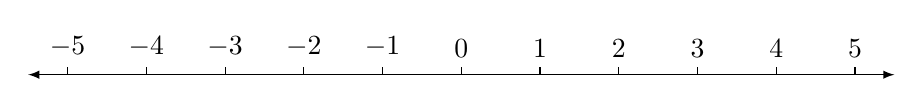
\begin{tikzpicture}
\draw[latex-latex] (-5.5, 0) -- (5.5, 0) ; 
\foreach \x in {-5,-4,-3,-2,-1,0,1,2,3,4,5} \draw (\x, 0) -- (\x, 0.1) node[above] {$\x$} ;
\end{tikzpicture}
\end{center}

This section will scrutinise the set of real numbers in its capacity as a \textit{complete ordered field}. Decomposing what this means:
\begin{itemize} 
\item A \textit{field} is a set with a notion of `zero' and `one', in which it makes sense to talk about addition, subtraction, multiplication, and division by everything except zero. Examples are $\mathbb{Q}$, $\mathbb{R}$, and $\mathbb{Z}/p\mathbb{Z}$ when $p$ is a prime number (but not when $p$ is composite). However, $\mathbb{Z}$ is not a field, since we can't freely divide by nonzero elements---for example, $1 \in \mathbb{Z}$ and $2 \in \mathbb{Z}$, but no integer $n$ satisfies $2n=1$.
\item An \textit{ordered field} is a field which is equipped with a well-behaved notion of order. Both $\mathbb{Q}$ and $\mathbb{R}$ are ordered fields, but $\mathbb{Z}/p\mathbb{Z}$ is not. We'll see why soon.
\item A \textit{complete ordered field} is an ordered field in which every set with an upper bound has a \textit{least} upper bound. As we will see, $\mathbb{Q}$ is not a complete ordered field, but $\mathbb{R}$ is.
\end{itemize}

This is made (extremely) precise in \Cref{secConstructions}.

\subsection*{Magnitude and scalar product}

In this part of the section, we home in on sets of the form $\mathbb{R}^n$, for $n \in \mathbb{N}$. Elements of $\mathbb{R}^n$ are sequences of the form $(x_1,x_2,\dots,x_n)$, where each $x_i \in \mathbb{R}$. With our interpretation of the reals $\mathbb{R}$ as a \textit{line}, we can interpret a sequence $(x_1,x_2,\dots,x_n)$ as a point in \textit{$n$-dimensional space}:
\begin{itemize}
\item $0$-dimensional space is a single point. The set $\mathbb{R}^0$ has one element, namely the empty sequence $()$, so this makes sense.
\item $1$-dimensional space is a line. This matches our intuition that $\mathbb{R}=\mathbb{R}^1$ forms a line.
\item $2$-dimensional space is a \textit{plane}. The elements of $\mathbb{R}^2$ are pairs $(x,y)$, where $x$ and $y$ are both real numbers. We can interpret the pair $(x,y)$ as \textit{coordinates} for a point which is situated $x$ units to the right of $(0,0)$ and $y$ units above $(0,0)$ (where negative values of $x$ or $y$ reverse this direction)---see \Cref{figPointsInR2}.
\end{itemize}

\begin{figure}[ht]
\centering
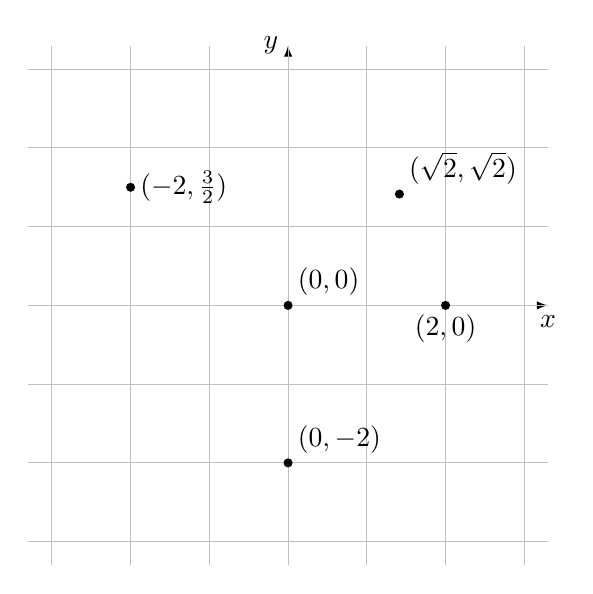
\begin{tikzpicture}
\draw[-latex] (-3.3, 0) -- (3.3, 0) node[below] {$x$} ;
\draw[-latex] (0, -3.3) -- (0, 3.3) node[left] {$y$} ;
\foreach \x in {-3,-2,-1,0,1,2,3} \draw[lightgray] (\x, -3.3) -- (\x, 3.3) ;
\foreach \y in {-3,-2,-1,0,1,2,3} \draw[lightgray] (-3.3, \y) -- (3.3, \y) ;
\draw[fill] (0,0) circle[radius=0.05] node[above right] {$(0,0)$} ;
\draw[fill] ({sqrt(2)},{sqrt(2)}) circle[radius=0.05] node[above right] {$(\sqrt{2},\sqrt{2})$} ;
\draw[fill] (0,-2) circle[radius=0.05] node[above right] {$(0,-2)$} ;
\draw[fill] (2,0) circle[radius=0.05] node[below] {$(2,0)$} ;
\draw[fill] (-2,1.5) circle[radius=0.05] node[right] {$(-2, \frac{3}{2})$} ;
\end{tikzpicture}
\caption{Some points in $\mathbb{R}^2$}
\label{figPointsInR2}
\end{figure}

With this intuition in mind, we set up the following notation.

\begin{notation}
\label{ntnVectorsInRn}
\index{origin}
\index{component}
Let $n \in \mathbb{N}$. Elements of $\mathbb{R}^n$ will be denoted $\vec x, \vec y, \vec z, \dots$\nindex{xvec}{$\vec x$}{vector} \inlatex{vec}\lindexmmc{vec}{$\vec a, \vec b, \dots$} and called ($n$-\textbf{dimensional}) \textbf{vectors}. Given a vector $\vec x \in \mathbb{R}^n$, we write $x_i$ for the $i^{\text{th}}$ \textbf{component} of $\vec x$, so that
\[ \vec x = (x_1,x_2,\dots,x_n) \]
The element $(0,0,\dots,0) \in \mathbb{R}^n$ is called the \textbf{origin} or \textbf{zero vector} of $\mathbb{R}^n$, and is denoted by $\vec 0$.

Moreover, if $\vec x, \vec y \in \mathbb{R}^n$ and $a \in \mathbb{R}$ we write
\[ \vec x + \vec y = (x_1+y_1,x_2+y_2,\dots,x_n+y_n) \quad \text{and} \quad a \vec x = (ax_1,ax_2,\dots,ax_n) \]
\end{notation}

\begin{example}
For all $\vec x \in \mathbb{R}^n$, we have
\[ \vec x + \vec 0 = \vec x \quad \text{and} \quad 1 \vec x = \vec x \]
\end{example}

\begin{definition}
\label{defMagnitude}
\index{magnitude}
\index{distance}
Let $\vec x \in \mathbb{R}^n$. The \textbf{magnitude} of $\vec x$ is the real number $\lVert \vec x \rVert$\nindex{xmag}{$\lVert \vec x \rVert$}{magnitude} \inlatex{lVert\ \textbackslash{}vec\ x\ \textbackslash{}rVert}\lindexmmc{lVert\dots{}\textbackslash{}rVert}{$\lVert \dots{} \rVert$} defined by
\[ \lVert \vec x \rVert = \sqrt{\sum_{i=1}^n x_i^2} = \sqrt{x_1^2+x_2^2+\cdots+x_n^2} \]
Given vectors $\vec x, \vec y \in \mathbb{R}^n$, the \textbf{distance} from $\vec x$ to $\vec y$ is defined to be $\lVert \vec y - \vec x \rVert$. Thus the magnitude of a vector can be thought of as the distance from that vector to the origin.
\end{definition}

\begin{example}
\label{exMagnitudeInR2}
In $\mathbb{R}^2$, \Cref{defMagnitude} says that
\[ \lVert (x,y) \rVert = \sqrt{x^2+y^2} \]
This matches the intuition obtained from the Pythagorean theorem on the sides of right-hand triangles. For example, consider the triangle with vertices $(0,0)$, $(4,0)$ and $(4,3)$:
\begin{center}
\begin{tikzpicture}
\draw (0,0) node [below left] {$(0,0)$}
   -- (4,0) node [below right] {$(4,0)$}
   -- (4,3) node [above right] {$(4,3)$}
   -- (0,0) ;
\end{tikzpicture}
\end{center}
The hypotenuse of the triangle has magnitude
\[ \lVert (4,3) \rVert = \sqrt{4^2+3^2} = \sqrt{25} = 5 \]
\end{example}

\begin{exercise}
\label{exDistanceIsSymmetric}
Let $\vec x, \vec y \in \mathbb{R}^n$. Prove that $\lVert \vec x - \vec y \rVert = \lVert \vec y - \vec x \rVert$. That is, the distance from $\vec x$ to $\vec y$ is equal to the distance from $\vec y$ to $\vec x$.
\end{exercise}

\begin{exercise}
Prove that if $x \in \mathbb{R}$ then the magnitude $\lVert (x) \rVert$ is equal to the absolute value $|x|$.
\end{exercise}

\begin{exercise}
\label{exVectorZeroIffMagnitudeZero}
Let $\vec x \in \mathbb{R}^n$. Prove that $\lVert \vec x \rVert = 0$ if and only if $\vec x = \vec 0$.
\end{exercise}

\subsection*{The triangle inequality and the Cauchy--Schwarz inequality}

The first, and simplest, inequality that we investigate is the (one-dimensional version of the) \textit{triangle inequality} (\Cref{thmTriangleInequality1D}). It is so named because of a generalisation to higher dimensions (\Cref{thmTriangleInequality}), which can be interpreted geometrically as saying that the sum of two side lengths of a triangle is greater than or equal to the third side length.

The triangle inequality is used very frequently in mathematical proofs---you will encounter it repeatedly in this chapter---yet its proof is surprisingly simple.

Before we can prove the triangle inequality, we need the following fact about square roots of real numbers.

\begin{lemma}
\label{lemSquareRootIsOrderPreserving}
Let $x,y \in \mathbb{R}$. If $0 \le x \le y$, then $\sqrt{x} \le \sqrt{y}$.
\end{lemma}
\begin{cproof}
Suppose $0 \le x \le y$. Note that, by definition of the square root symbol, we have $\sqrt{x} \ge 0$ and $\sqrt{y} \ge 0$.

Suppose $\sqrt{x} > \sqrt{y}$. By two applications of \Cref{thmPropertiesOfOrderedFields}(d), we have
\[ y = \sqrt{y} \cdot \sqrt{y} < \sqrt{x} \cdot \sqrt{y} < \sqrt{x} \cdot \sqrt{x} = x \]
so that $y<x$. But this contradicts the assumption that $x \le y$. Hence $\sqrt{x} \le \sqrt{y}$, as required.
\end{cproof}

\begin{theorem}[Triangle inequality in one dimension]
\label{thmTriangleInequality1D}
\index{triangle inequality!in one dimension}
\index{inequality!triangle (one-dimensional)}
Let $x,y \in \mathbb{R}$. Then $|x+y| \le |x|+|y|$. Moreover, $|x+y|=|x|+|y|$ if and only if $x$ and $y$ have the same sign.
\end{theorem}
\begin{cproof}
Note first that $xy \le |xy|$; indeed, $xy$ and $|xy|$ are equal if $xy$ is non-negative, and otherwise we have $xy < 0 < |xy|$. Also $x^2=|x|^2$ and $y^2=|y|^2$. Hence
\[ (x+y)^2 = x^2+2xy+y^2 \le |x|^2+2|xy|+|y|^2 = (|x|+|y|)^2 \]
Taking (nonnegative) square roots yields
\[ |x+y| \le ||x|+|y|| \]
by \Cref{lemSquareRootIsOrderPreserving}. But $|x|+|y| \ge 0$, so $||x|+|y||=|x|+|y|$. This completes the first part of the proof.

Equality holds in the above if and only if $xy=|xy|$, which occurs if and only if $xy \ge 0$. But this is true if and only if $x$ and $y$ are both non-negative or both non-positive---that is, they have the same sign.
\end{cproof}

\begin{example}
Let $x,y \in \mathbb{R}$. We prove that
\[ \frac{|x+y|}{1+|x+y|} \le \frac{|x|}{1+|x|} + \frac{|y|}{1+|y|} \]
First note that, if $0 \le s \le t$, then
\[ \frac{s}{1+s} \le \frac{t}{1+t} \]
To see this, note that
\begin{align*}
s \le t &\Rightarrow 1+s \le 1+t && \text{rearranging} \\
&\Rightarrow \frac{1}{1+t} \le \frac{1}{1+s} && \text{since $1+s,1+t > 0$} \\
&\Rightarrow 1-\frac{1}{1+s} \le 1-\frac{1}{1+t} && \text{rearranging} \\
&\Rightarrow \frac{s}{1+s} \le \frac{t}{1+t} && \text{rearranging}
\end{align*}
Now letting $s=|x+y|$ and $t=|x|+|y|$, we have $s \le t$ by the triangle inequality, and hence
\[ \frac{|x+y|}{1+|x+y|} \le \frac{|x|}{{1+|x|+|y|}} + \frac{|y|}{1+|x|+|y|} \le \frac{|x|}{1+|x|} + \frac{|y|}{1+|y|} \]
as required.
\end{example}

\begin{exercise}
Let $n \in \mathbb{N}$ and let $x_i \in \mathbb{R}$ for each $i \in [n]$. Prove that
\[ \left| \sum_{i=1}^n x_i \right| \le \sum_{i=1}^n |x_i| \]
with equality if and only if the numbers $x_i$ are either all non-positive or all non-negative.
\end{exercise}

\begin{exercise}
Let $x,y \in \mathbb{R}$. Prove that
\[ ||x|-|y|| \le |x-y| \]
\end{exercise}

We will generalise the triangle inequality to arbitrary dimensions in \Cref{thmTriangleInequality}. Our proof will go via the \textit{Cauchy--Schwarz inequality} (\Cref{thmCauchySchwarzInequality}). To motivate the Cauchy--Schwarz inequality, we introduce another geometric notion called the \textit{scalar product} of two vectors.

\begin{definition}
\label{defScalarProduct}
\index{scalar product}
\index{dot product}
Let $\vec x,\vec y \in \mathbb{R}^n$. The \textbf{scalar product} (or \textbf{dot product}) of $\vec x$ with $\vec y$ is the real number $\vec x \cdot \vec y$\nindex{xdoty}{$\vec x \cdot \vec y$}{scalar product} \inlatex{cdot}\lindexmmc{cdot}{$\cdot$} defined by
\[ \vec x \cdot \vec y = \sum_{i=1}^n x_iy_i = x_1y_1+x_2y_2+\cdots+x_ny_n \]
\end{definition}

\begin{example}
\label{exVectorDotItself}
Let $\vec x \in \mathbb{R}^n$. Then $\vec x \cdot \vec x = \lVert \vec x \rVert^2$. Indeed
\[ \vec x \cdot \vec x = \sum_{i=1}^n x_i^2 = \lVert \vec x \rVert^2 \]
\end{example}

\begin{exercise}
\label{exScalarProductIsBilinear}
Let $\vec x, \vec y, \vec z, \vec w \in \mathbb{R}^n$ and let $a,b,c,d \in \mathbb{R}$. Prove that
\[ (a \vec x + b \vec y) \cdot (c \vec z + d \vec w) = ac (\vec x \cdot \vec z) + ad (\vec x \cdot \vec w) + bc( \vec y \cdot \vec z) + bd (\vec y \cdot \vec w) \]
\end{exercise}

Intuitively, the scalar product of two vectors $\vec x$ and $\vec y$ measures the extent to which $\vec x$ and $\vec y$ fail to be \textit{orthogonal}. In fact, if $\theta$ is the acute angle formed between the lines $\ell_1$ and $\ell_2$, where $\ell_1$ passes through $\vec 0$ and $\vec x$ and $\ell_2$ passes through $\vec 0$ and $\vec y$, then a formula for the scalar product of $\vec x$ and $\vec y$ is given by
\[ \vec x \cdot \vec y = \lVert \vec x \rVert \lVert \vec y \rVert \cos \theta \]

\begin{center}
\begin{tikzpicture}[scale=1.5]
\draw [->] (0,0) node [left] {$\vec 0$}
        -- (4,2) node [above right] {$\vec x$} ;
\draw [->] (0,0)
        -- (5,0) node [right] {$\vec y$} ;
\draw [dashed] (4,2) -- (4,0) ;
\draw (3.7,0) -- (3.7,0.3) -- (4,0.3) ;
\draw [<->] (0,-0.3) -- (4,-0.3) ;
\node [below] at (2,-0.3) {$\lVert x \rVert \cos \theta$} ;
\draw [->, domain=0:atan(0.5)] plot ({0.7*cos(\x)},{0.7*sin(\x)}) ;
\node at ({0.85*cos(atan(0.25))}, {0.85*sin(atan(0.25))}) {$\theta$} ;
\end{tikzpicture}
\end{center}

Evidently, $\vec x$ and $\vec y$ are orthogonal if and only if $\cos \theta = 0$, in which case $\vec x \cdot \vec y = 0$ as well. We cannot prove this yet, though, as we have not yet defined trigonometric functions or explored their properties, but hopefully this provides some useful intuition.

The Cauchy--Schwarz inequality provides a useful comparison of the size of a scalar product of two vectors with the magnitudes of the vectors.

\begin{theorem}[Cauchy--Schwarz inequality]
\label{thmCauchySchwarzInequality}
\index{Cauchy--Schwarz inequality}
\index{inequality!Cauchy--Schwarz}
Let $n \in \mathbb{N}$ and let $x_i,y_i \in \mathbb{R}$ for each $i \in [n]$. Then
\[ |\vec x \cdot \vec y| \le \lVert \vec x \rVert \lVert \vec y \rVert \]
with equality if and only if $a\vec x = b\vec y$ for some $a,b \in \mathbb{R}$ which are not both zero.
\end{theorem}
\begin{cproof}
If $\vec y = \vec 0$, then this is trivial: both sides of the equation are equal to zero! So assume that $\vec y \ne \vec 0$. In particular, by \Cref{exVectorZeroIffMagnitudeZero}, we have $\lVert \vec y \rVert > 0$.

Define $k = \dfrac{\vec x \cdot \vec y}{\lVert \vec y \rVert^2}$. Then
\begin{align*}
0 &\le \lVert \vec x - k \vec y \rVert^2 && \text{since squares are nonnegative} \\
&= (\vec x - k \vec y) \cdot (\vec x - k \vec y) && \text{by \Cref{exVectorDotItself}} \\
&= (\vec x \cdot \vec x) - 2k (\vec x \cdot \vec y) + k^2 (\vec y \cdot \vec y) && \text{by \Cref{exScalarProductIsBilinear}} \\
&= \lVert \vec x \rVert^2 - \frac{(\vec x \cdot \vec y)^2}{\lVert y \rVert^2} && \text{by definition of $k$}
\end{align*}
Multiplying through by $\lVert \vec y \rVert^2$, which is non-negative and therefore doesn't change the sign of the inequality, yields
\[ 0 \le \lVert \vec x \rVert^2 \lVert \vec y \rVert^2 - (\vec x \cdot \vec y)^2 \]
which is equivalent to what was to be proved.

Evidently, equality holds if and only if $\lVert \vec x - k \vec y \rVert = 0$, which by \Cref{exVectorZeroIffMagnitudeZero} occurs if and only if $\vec x - k \vec y = 0$. Now:
\begin{itemize}
\item If $\vec x - k\vec y = 0$, then we have
\begin{align*}
&\vec x - k \vec y = 0 && \\
&\Leftrightarrow \vec x - \frac{\vec x \cdot \vec y}{\lVert \vec y \rVert^2} \vec y = 0 && \text{by definition of $k$} \\
&\Leftrightarrow \lVert \vec y \rVert^2 \vec x = (\vec x \cdot \vec y) \vec y && \text{rearranging}
\end{align*}
%% BEGIN EXTRACT (xtrProvingExistsExampleTwo) %%
If $\vec y \ne \vec 0$ then let $a=\lVert \vec y \rVert^2$ and $b=\vec x \cdot \vec y$; otherwise, let $a=0$ and $b=1$. In both cases, we have $a \vec x = b \vec y$ and $a,b$ are not both zero.
%% END EXTRACT %%

If $a \vec x = b \vec y$ for some $a,b \in \mathbb{R}$ not both zero, then either:
\begin{itemize}
\item $a=0$ and $b \ne 0$, in which case $\vec y = 0$ and we have equality in the Cauchy--Schwarz inequality; or
\item $a \ne 0$, in which case $\vec y = \frac{b}{a} \vec x$. Write $c=\frac{b}{a}$. Then
\begin{align*}
|\vec x \cdot \vec y| &= | \vec x \cdot (c \vec x) | && \\
&= |c(\vec x \cdot \vec x)| && \text{by \Cref{exScalarProductIsBilinear}} \\
&= |c| \lVert \vec x \rVert^2 && \text{by \Cref{exVectorDotItself}} \\
&= \lVert \vec x \rVert \lVert c \vec x \rVert && \text{rearranging} \\
&= \lVert \vec x \rVert \lVert \vec y \rVert &&
\end{align*}
\end{itemize}
In either case, we have equality in the Cauchy--Schwarz inequality.
\end{itemize}

So equality holds if and only if $a \vec x = b \vec y$ for some $a,b \in \mathbb{R}$ not both zero.
\end{cproof}

\begin{example}
Let $a,b,c \in \mathbb{R}$. We'll prove that
\[ ab+bc+ca \le a^2+b^2+c^2 \]
and examine when equality holds.

Letting $\vec x = (a,b,c)$ and $\vec y = (b,c,a)$ yields
\[ \vec x \cdot \vec y = ab+bc+ca \]
and
\[ \lVert \vec x \rVert = \sqrt{a^2+b^2+c^2} = \sqrt{b^2+c^2+a^2} = \lVert \vec y \rVert \]
Hence $\lVert \vec x \rVert \lVert \vec y \rVert = a^2+b^2+c^2$. By the Cauchy--Schwarz inequality, it follows that
\[ \vec x \cdot \vec y = ab+bc+ca \le a^2+b^2+c^2 = \lVert \vec x \rVert \lVert \vec y \rVert \]
as required. Equality holds if and only if $k(a,b,c) = \ell(b,c,a)$ for some $k,\ell \in \mathbb{R}$ not both zero. We may assume $k \ne 0$---otherwise, swap the vectors $\vec x$ and $\vec y$ in what follows. Then, letting $t=\frac{\ell}{k}$, we have
\begin{align*}
&k(a,b,c) = \ell(b,c,a) && \\
&\Leftrightarrow (a,b,c) = (tb,tc,ta) && \text{by definition of $t$} \\
&\Leftrightarrow (a,b,c) = (t^2c,t^2a,t^2b) && \text{substituting $a=tb$ etc.} \\
&\Leftrightarrow (a,b,c) = (t^3a,t^3b,t^3c) && \text{substituting $a=tb$ etc.\ again} \\
&\Leftrightarrow \vec x = t^3 \vec x
\end{align*}
This occurs if and only if either $(a,b,c)=(0,0,0)$, or $t=1$, in which case
\[ (a,b,c) = (tb,tc,ta) = (b,c,a) \]
So equality holds if and only if $a=b=c$.
\end{example}

\begin{exercise}
Let $r \in \mathbb{N}$ and let $a_1,a_2,\dots,a_r \in \mathbb{R}$ be such that $a_1^2+a_2^2+\cdots+a_n^2=6$. Prove that
\[ (a_1+2a_2+\cdots+na_n)^2 \le n(n+1)(2n+1) \]
and determine when equality holds.
\end{exercise}

We now use the Cauchy--Schwarz inequality to generalise the one-dimensional version of the triangle inequality (\Cref{thmTriangleInequality1D}) to arbitrary (finite) dimensions.

\begin{theorem}[Triangle inequality]
\label{thmTriangleInequality}
\index{triangle inequality}
\index{inequality!triangle}
Let $\vec x, \vec y \in \mathbb{R}^n$. Then
\[ \lVert \vec x + \vec y \rVert \le \lVert \vec x \rVert + \lVert \vec y \rVert \]
with equality if and only if $a\vec x = b\vec y$ for some real numbers $a,b \ge 0$.
\end{theorem}

\begin{cproof}
We proceed by calculation:
\begin{align*}
\lVert \vec x + \vec y \rVert^2
&= (\vec x + \vec y) \cdot (\vec x + \vec y) && \text{by \Cref{exVectorDotItself}} \\
&= (\vec x \cdot \vec x) + 2(\vec x \cdot \vec y) + (\vec y \cdot \vec y) && \text{by \Cref{exScalarProductIsBilinear}} \\
&\le (\vec x \cdot \vec x) + 2|\vec x \cdot \vec y| + (\vec y \cdot \vec y) && \text{since $a \le |a|$ for all $a \in \mathbb{R}$} \\
&\le \lVert \vec x \rVert^2 + 2\lVert x \rVert \lVert y \rVert + \lVert \vec y \rVert^2 && \text{by \Cref{exVectorDotItself} and Cauchy--Schwarz} \\
&= (\lVert \vec x \rVert + \lVert \vec y \rVert)^2 && \text{rearranging}
\end{align*}

Taking (nonnegative) square roots of both sides yields
\[ \lVert \vec x + \vec y \rVert \le \lVert \vec x \rVert + \lVert \vec y \rVert \]
by \Cref{lemSquareRootIsOrderPreserving}, as required.

Equality holds if and only if the two `$\le$' symbols in the above derivation are in fact `$=$' symbols.
\begin{itemize}
\item The first inequality is equality if and only if $\vec x \cdot \vec y = |\vec x \cdot \vec y|$, which holds if and only if $\vec x \cdot \vec y \ge 0$.
\item The second inequality is equality if and only if equality holds in the Cauchy--Schwarz inequality. In turn, this occurs if and only if $a\vec x = b \vec y$ for some $a,b \in \mathbb{R}$. We may, moreover, assume that $a \ge 0$---if not, replace $a$ and $b$ by their negatives.
\end{itemize}
If $a=0$ then we can take $b=0$.
%% BEGIN EXTRACT {xtrSoExampleTwo} %%
If $a>0$, then by \Cref{exVectorDotItself} and \Cref{exScalarProductIsBilinear}, we have
\[ \vec x \cdot \left( \frac{b}{a} \vec x \right) = \frac{b}{a} \lVert \vec x \rVert^2 \]
which is non-negative if and only if $b \ge 0$, since we are assuming that $a \ge 0$.
%% END EXTRACT %%

Thus, equality holds in the triangle inequality if and only if $a\vec x = b\vec y$ for some $a,b \ge 0$.
\end{cproof}

This general version of the triangle inequality has a geometric interpretation in terms of---you guessed it---triangles. Any three points $\vec a, \vec b, \vec c \in \mathbb{R}^n$ form a (potentially flat) triangle:

\begin{center}
\begin{tikzpicture}
\draw (0,2) -- (7,0) node[pos=0, left] {$\vec a$}
                     node[midway, below left] {$u$}
            -- (3,4) node[pos=0, right] {$\vec b$}
                     node[midway, above right] {$v$}
            -- (0,2) node[pos=0, above] {$\vec c$}
                     node[midway, above left] {$w$};
\end{tikzpicture}
\end{center}

The side lengths $u,v,w$ are given by the following equations:
\[ u = \lVert \vec b - \vec a \rVert, \quad v = \lVert \vec c - \vec b \rVert, \quad w = \lVert \vec a - \vec c \rVert \]
The triangle inequality says tells us that $u \le v + w$. Indeed:
\begin{align*}
u &= \lVert \vec b - \vec a \rVert && \text{by definition of $u$} \\
&= \lVert (\vec b - \vec c) + (\vec c - \vec a) \rVert && \text{rearranging} \\
&\le \lVert \vec b - \vec c \rVert + \lVert \vec c - \vec a \rVert && \text{by the triangle inequality} \\
&= \lVert \vec c - \vec b \rVert + \lVert \vec a - \vec c \rVert && \text{by \Cref{exDistanceIsSymmetric}} \\
&= v + w && \text{by definition of $v$ and $w$}
\end{align*}

That is, the triangle inequality says that the sum of two side lengths of a triangle is greater than or equal to the third side length. Moreover, it tells us $u=v+w$ precisely when $k(\vec a - \vec c) = \ell(\vec c - \vec b)$ for some $k,\ell \ge 0$. If $k=0$ then
\[ \vec c \quad = \quad \vec b \quad = \quad 0 \vec a + (1-0) \vec b \]
if $k>0$, then $k+\ell>0$, so we have
\[ \vec c \quad = \quad \frac{k}{k+\ell} \vec a + \frac{\ell}{k+\ell} \vec b \quad = \quad \frac{k}{k+\ell} \vec a + \left( 1 - \frac{k}{k+\ell} \right)\vec b \]
Examining this a bit more closely yields that $u=v+w$ if and only if
\[ \vec c = t\vec a + (1-t) \vec b \]
for some $0 \le t \le 1$, which is to say precisely that $\vec c$ lies on the line segment between $\vec a$ and $\vec b$. In other words, equality holds in the triangle inequality only if the three vertices of the triangle are \textit{collinear}, which is to say that the triangle whose vertices are the points $\vec a$, $\vec b$ and $\vec c$, is flat.

\subsection*{Inequalities of means}

Our goal now is to explore different kinds of average---specifically, \textit{means}---of finite sets of non-negative real numbers. We will compare the relative sizes of these means with respect to one-another, with emphasis on three particular kinds of mean: the \textit{arithmetic mean} (\Cref{defArithmeticMean}), the \textit{geometric mean} (\Cref{defGeometricMean}) and the \textit{harmonic mean} (\Cref{defHarmonicMean}). These means in fact assemble into a continuum of means, called \textit{generalised means} (\Cref{defGeneralisedMean}), all of which can be compared with one another.

\begin{definition}
\label{defArithmeticMean}
\index{mean!arithmetic}
Let $n \ge 1$. The (\textbf{arithmetic}) \textbf{mean} of real numbers $x_1,\dots,x_n$ is
\[ \frac{1}{n} \sum_{i=1}^n x_i = \frac{x_1 + x_2 + \cdots + x_n}{n} \]
\end{definition}

\begin{definition}
\label{defGeometricMean}
\index{mean!geometric}
Let $n \ge 1$. The \textbf{geometric mean} of non-negative real numbers $x_1,\dots,x_n$ is
\[ \sqrt[n]{\prod_{i=1}^n x_i} = \sqrt[n]{x_1 \cdot x_2 \cdot \dots \cdot x_n} \]
\end{definition}

The following theorem is commonly known as the \textbf{AM--GM inequality}.

\begin{theorem}[Inequality of arithmetic and geometric means]
\label{thmAMGMInequality}
\index{AM--GM inequality}
\index{inequality!of arithmetic and harmonic means}
Let $n \in \mathbb{N}$ and $x_1,x_2,\dots,x_n \ge 0$. Then
\[ \underbrace{\sqrt[n]{x_1 \cdots x_n}}_{\text{geometric mean}} \le \underbrace{\frac{x_1 + \cdots + x_n}{n}}_{\text{arithmetic mean}} \]
with equality if and only if $x_1 = \cdots = x_n$.
\end{theorem}
\begin{cproof}[when $n=2$]
We need to show that, if $x,y \in \mathbb{R}$ with $x, y \ge 0$, then
\[ \sqrt{xy} \le \frac{x+y}{2} \]
with equality if and only if $x=y$.

First note that the square roots of $x$ and $y$ exist since they are non-negative. Now
\begin{align*}
0 &\le (\sqrt{x}-\sqrt{y})^2 && \text{since squares are nonnegative} \\
&= (\sqrt{x})^2 - 2\sqrt{x}\sqrt{y} + (\sqrt{y})^2 && \text{expanding} \\
&= x - 2\sqrt{xy} + y && \text{rearranging}
\end{align*}

Rearranging the inequality $0 \le x-2\sqrt{xy}+y$ yields the desired result.

If $\sqrt{xy} = \frac{x+y}{2}$, then we can rearrange the equation as follows:
\begin{align*}
\sqrt{xy} = \frac{x+y}{2} &\Rightarrow 2\sqrt{xy} = x+y && \text{multiplying by $2$} \\
&\Rightarrow 4xy = x^2+2xy+y^2 && \text{squaring both sides} \\
&\Rightarrow x^2-2xy+y^2 = 0 && \text{rearranging} \\
&\Rightarrow (x-y)^2 = 0 && \text{factorising} \\
&\Rightarrow x-y = 0 && \text{since $a^2=0 \Rightarrow a=0$ for $a \in \mathbb{R}$} \\
&\Rightarrow x=y && \text{rearranging}
\end{align*}
So we have proved both parts of the theorem.
\end{cproof}

\begin{example}
We use the AM--GM inequality to prove that the area of a rectangle with fixed perimeter is maximised when the rectangle is a square.

Indeed, fix a perimeter $p > 0$, and let $x,y > 0$ be side lengths of a rectangle with perimeter $p$---that is, $x$ and $y$ satisfy the equation $2x+2y=p$. The area $a$ of the rectangle satisfies $a=xy$. By the AM--GM inequality, we have
\[ a = xy \le \left( \frac{x+y}{2} \right)^2 = \frac{p^2}{16} \]
Equality holds if and only if $x=y$, in other words, if and only if the rectangle is a square.
\end{example}

\begin{exercise}
Let $a,b > 0$ be real numbers. Prove that $\displaystyle \frac{a^2+b^2}{2} \ge ab$.
\end{exercise}

\begin{example}
Let $x>0$. We find the minimum possible value of $x+\frac{9}{x}$. By the AM--GM inequality, we have
\[ x+\frac{9}{x} \ge 2\sqrt{x \cdot \frac{9}{x}} = 2 \sqrt{9} = 6 \]
with equality if and only if $x=\frac{9}{x}$, which occurs if and only if $x=3$. Hence the minimum value of $x+\frac{9}{x}$ when $x>0$ is $6$.
\end{example}

\begin{exercise}
Let $x>0$ and let $n \in \mathbb{N}$. Find the minimum possible value of $\displaystyle \sum_{k=-n}^n x^k$.
\end{exercise}

\Cref{exAMGMForPowersOf2,exAMGMForPredecessors} complete the proof of the AM--GM inequality (\Cref{thmAMGMInequality}). Before proceeding with the exercises, let's fix some notation: for each $n \in \mathbb{N}$, let $p_{\text{AM--GM}}(n)$ be the assertion that
the AM--GM inequality holds for collections of $n$ numbers; that is, $p_{\text{AM--GM}}(n)$ is the assertion:
\begin{quote}
For all $x_1,x_2,\dots,x_n \ge 0$, we have
\[ \sqrt[n]{\prod_{i=1}^n x_i} \le \frac{1}{n} \sum_{i=1}^n x_i \]
with equality if and only if $x_1=x_2=\cdots=x_n$.
\end{quote}
Note that we already proved $p_{\text{AM--GM}}(2)$.

\begin{exercise}
\label{exAMGMForPowersOf2}
Let $r \in \mathbb{N}$ and let $x_1,x_2,\dots,x_{2r} \in \mathbb{R}$. Write
\[ a = \frac{1}{r} \sum_{i=1}^r x_i \quad \text{and} \quad g = \sqrt[r]{\prod_{i=1}^r x_i} \]
for the arithmetic and geometric means, respectively, of the numbers $x_1,\dots,x_r$; write
\[ a' = \frac{1}{r} \sum_{i=r+1}^{2r} x_i \quad \text{and} \quad g' = \sqrt[r]{\prod_{i=r+1}^{2r} x_i} \]
for the arithmetic and geometric means, respectively, of the numbers $x_{r+1},\dots,x_{2r}$; and write
\[ A = \frac{1}{2r} \sum_{i=1}^{2r} x_i \quad \text{and} \quad G = \sqrt[2r]{\prod_{i=1}^{2r} x_i} \]
for the arithmetic and geometric means, respectively, of all the numbers $x_1,\dots,x_{2r}$.

Prove that
\[ A = \frac{a+a'}{2} \quad \text{and} \quad G=\sqrt{gg'} \]
Deduce that, for each $r \in \mathbb{N}$, if $p_{\text{AM--GM}}(r)$ is true then $p_{\text{AM--GM}}(2r)$ is true. Deduce further than $p_{\text{AM--GM}}(2^m)$ is true for all $m \in \mathbb{N}$.
\end{exercise}

\begin{exercise}
\label{exAMGMForPredecessors}
Let $r \ge 2$ and let $x_1,\dots,x_{r-1} \in \mathbb{N}$. Define
\[ x_r = \frac{1}{r-1} \sum_{i=1}^{r-1} x_i \]
Prove that
\[ \frac{1}{r}\sum_{i=1}^r x_i = x_r \]
Assuming $p_{\text{AM--GM}}(r)$, deduce that
\[ x_r^r \ge \prod_{i=1}^r x_i = \left(\prod_{i=1}^{r-1} x_i\right) \cdot x_r \]
with equality if and only if $x_1=x_2=\cdots=x_r$. Deduce that $p_{\text{AM--GM}}(r)$ implies $p_{\text{AM--GM}}(r-1)$. Use \Cref{exAMGMForPowersOf2} to deduce further that $p_{\text{AM--GM}}(n)$ is true for all $n \ge 1$.
\end{exercise}

We now introduce another kind of mean, called the \textit{harmonic mean}.

\begin{definition}
\label{defHarmonicMean}
\index{mean!harmonic}
Let $n \in \mathbb{N}$. The \textbf{harmonic mean} of nonzero real numbers $x_1,x_2,\dots,x_n$ is
\[ \left( \frac{1}{n} \sum_{i=1}^n x_i^{-1} \right)^{-1} = \cfrac{n}{\frac{1}{x_1} + \frac{1}{x_2} + \cdots + \frac{1}{x_n}} \]
\end{definition}

The harmonic mean of two nonzero real numbers $x$ and $y$ has a simpler expression:
\[ \left( \frac{x^{-1}+y^{-1}}{2} \right)^{-1} = \frac{2xy}{x+y} \]

The harmonic mean arises naturally when considering rates of change of quantities over fixed amounts of time.

\begin{example}
The cities of York and Leeds are located $d>0$ miles apart. Two cars drive from York to Leeds, then immediately turn around and drive back. The two cars depart from York at the same time and arrive back in York at the same time.
\begin{itemize}
\item The first car drives from York to Leeds at a constant speed of $u$ miles per hour, and drives back to York at a constant speed of $v$ miles per hour.
\item The second car drives from York to Leeds and back again at the same constant speed of $w$ miles per hour.
\end{itemize}
According to the following formula from physics:
\[ \text{speed} \times \text{time} = \text{distance} \]
the time spent driving by the first car is $\frac{d}{u} + \frac{d}{v}$, and the time spent driving by the second car is $\frac{2d}{w}$.

Since the cars spend the same amount of time driving, it follows that
\[ \frac{2d}{w} = \frac{d}{u} + \frac{d}{v} \qquad \Rightarrow \qquad w = \frac{2uv}{u+v} \]
That is, the second car's speed is the harmonic mean of the two speeds driven by the first car.
\end{example}

As might be expected, we now prove a theorem relating the harmonic means with the other means we have established so far---this theorem is known as the \textbf{GM--HM inequality}.

\begin{theorem}[Inequality of geometric and harmonic means]
\label{thmGMHMInequality}
\index{GM--HM inequality}
\index{inequality!of geometric and harmonic means}
Let $n \in \mathbb{N}$ and $x_1,x_2,\dots,x_n > 0$. Then
\[ \underbrace{\cfrac{n}{\frac{1}{x_1} + \frac{1}{x_2} + \cdots + \frac{1}{x_n}}}_{\text{harmonic mean}} \le \underbrace{\sqrt[n]{x_1x_2 \cdots x_n}}_{\text{geometric mean}} \]
with equality if and only if $x_1 = \cdots = x_n$.
\end{theorem}
\begin{cproof}[when $n=2$]
We need to prove that if $x,y > 0$, then
\[ \frac{2}{\frac{1}{x} + \frac{1}{y}} \le \sqrt{xy} \]
This is almost immediate from the AM--GM inequality (\Cref{thmAMGMInequality}). Indeed, since all numbers in sight are positive, we can take reciprocals to see that this inequality is equivalent to the assertion that
\[ \frac{1}{\sqrt{xy}} \le \frac{x^{-1} + y^{-1}}{2} \]
But $\frac{1}{\sqrt{xy}} = \sqrt{x^{-1}y^{-1}}$, so this is immediate from the AM--GM inequality.
\end{cproof}

\begin{exercise}
Prove the GM--HM inequality for general values of $n \in \mathbb{N}$.
\end{exercise}

Another example of a mean that has applications in probability theory and statistics is that of the \textit{quadratic mean}.

\begin{definition}
\label{defQuadraticMean}
\index{mean!quadratic}
\index{root-mean-square}
Let $n \in \mathbb{N}$. The \textbf{quadratic mean} (or \textbf{root-mean-square}) of real numbers $x_1,x_2,\dots,x_n$ is
\[ \left( \frac{1}{n} \sum_{i=1}^n x_i^2 \right)^{\frac{1}{2}} = \sqrt{\frac{x_1^2+x_2^2+\cdots+x_n^2}{n}} \]
\end{definition}

The following theorem is, predictably, known as the \textbf{QM--AM inequality} (or \textbf{RMS--AM inequality}); it is a nice application of the Cauchy--Schwarz inequality.

\begin{theorem}[Inequality of quadratic and arithmetic means]
\label{thmQMAMInequality}
\index{QM--AM inequality}
\index{inequality!of quadratic and arithmetic means}
Let $n > 0$ and $x_1,x_2,\dots,x_n \ge 0$. Then
\[ \underbrace{\frac{x_1 + \cdots + x_n}{n}}_{\text{arithmetic mean}} \le \underbrace{\sqrt{\frac{x_1^2+x_2^2+\cdots+x_n^2}{n}}}_{\text{quadratic mean}} \]
with equality if and only if $x_1 = \cdots = x_n$.
\end{theorem}

\begin{cproof}
Define
\[ \vec x = (x_1,x_2,\dots,x_n) \quad \text{and} \quad \vec y = (1,1,\dots,1) \]
Then
\begin{align*}
x_1+x_2+\cdots+x_n
&= \vec x \cdot \vec y && \text{by definition of scalar product} \\
&\le \lVert \vec x \rVert \lVert \vec y \rVert && \text{by Cauchy--Schwarz} \\
&= \sqrt{x_1^2+x_2^2+\cdots+x_n^2} \cdot \sqrt{n} && \text{evaluating the magnitudes}
\end{align*}
Dividing through by $n$ yields
\[ \frac{x_1+x_2+\cdots+x_n}{n} \le \sqrt{\frac{x_1^2+x_2^2+\cdots+x_n^2}{n}} \]
as required. Equality holds if and only if equality holds in the Cauchy--Schwarz inequality, which occurs if and only if
\[ (ax_1,ax_2,\dots,ax_n)=(b,b,\dots,b) \]
for some $a,b \in \mathbb{R}$ not both zero. If $a=0$ then $b=0$, so we must have $a \ne 0$. Hence equality holds if and only if $x_i=\frac{b}{a}$ for all $i \in [n]$---in particular, if and only if $x_1=x_2=\cdots=x_n$.
\end{cproof}

To summarise, what we have proved so far is
\[ \begin{matrix} \text{harmonic} \\ \text{mean} \end{matrix} \quad \overset{(\ref{thmGMHMInequality})}{\le} \quad \begin{matrix} \text{geometric} \\ \text{mean} \end{matrix} \quad \overset{(\ref{thmAMGMInequality})}{\le} \quad \begin{matrix} \text{arithmetic} \\ \text{mean} \end{matrix} \quad \overset{(\ref{thmQMAMInequality})}{\le} \quad \begin{matrix} \text{quadratic} \\ \text{mean} \end{matrix} \]
with equality in each case if and only if the real numbers whose means we are taking are all equal.

The following exercise allows us to bookend our chain of inequalities with the minimum and maximum of the collections of numbers.

\begin{exercise}
\label{exMinMeanMaxInequalities}
Let $n > 0$ and let $x_1,x_2,\dots,x_n$ be positive real numbers. Prove that
\[ \mathrm{min} \{ x_1,x_2,\dots,x_n \} \le \left( \frac{1}{n} \sum_{i=1}^n x_i^{-1} \right)^{-1} \quad \text{and} \quad \mathrm{max} \{ x_1,x_2,\dots,x_n \} \ge \left( \frac{1}{n} \sum_{i=1}^n x_i^2 \right)^{\frac{1}{2}} \]
with equality in each case if and only if $x_1=x_2=\cdots=x_n$.
\end{exercise}

\subsection*{\optmark{Generalised means}}

We conclude this section by mentioning a generalisation of the results we have proved about means. We are not yet ready to prove the results that we mention; they are only here for the sake of interest.

\begin{definition}
\label{defExtendedRealLine}
\index{extended real number line}
The \textbf{extended real number line} is the (ordered) set $[-\infty, \infty]$, defined by
\[ [-\infty,\infty] = \mathbb{R} \cup \{ -\infty, \infty \} \]
where $\mathbb{R}$ is the set of real numbers with its usual ordering, and $-\infty,\infty$ are new elements ordered in such a way that $-\infty < x < \infty$ for all $x \in \mathbb{R}$.
\end{definition}

Note that the extended real line does \textit{not} form a field---the arithmetic operations are not defined on $-\infty$ or $\infty$, and we will at no point treat $-\infty$ and $\infty$ as real numbers; they are merely elements which extend the reals to add a least element and a greatest element.

\begin{definition}
\label{defGeneralisedMean}
\index{mean!generalised}
Let $p \in [-\infty,\infty]$, let $n \in \mathbb{N}$, and let $x_1,x_2,\dots,x_n$ be positive real numbers. The \textbf{generalised mean with exponent $p$} (or simply $p$-\textbf{mean}) $x_1,x_2,\dots,x_n$ is the real number $M_p(x_1,x_2,\dots,x_n)$ defined by
\[ M_p(x_1,x_2,\dots,x_n) = \left( \frac{1}{n} \sum_{i=1}^n x_i^p \right)^{\frac{1}{p}} \]
if $p \not \in \{ -\infty, 0, \infty \}$, and by
\[ M_p(x_1,x_2,\dots,x_n) = \lim_{q \to p} M_q(x_1,x_2,\dots,x_n) \]
if $p \in \{ -\infty, 0, \infty \}$, where the notation $\lim\limits_{q \to p}$ refers to the \textit{limit} as $q$ tends to $p$, as discussed in \Cref{secLimitsOfFunctions}.
\end{definition}

We can see immediately that the harmonic, arithmetic and quadratic means of a finite set of positive real numbers are the $p$-means for a suitable value of $p$: the harmonic mean is the $(-1)$-mean, the arithmetic mean is the $1$-mean, and the quadratic mean is the $2$-mean. Furthermore, \Cref{propZeroAndInfinityMeans} exhibits the \textit{minimum} as the $(-\infty)$-mean, the \textit{geometric mean} as the $0$-mean, and the \textit{maximum} as the $\infty$-mean.

\begin{proposition}
\label{propZeroAndInfinityMeans}
Let $n > 0$ and let $x_1,x_2,\dots,x_n \ge 0$. Then
\begin{itemize}
\item $M_{-\infty}(x_1,x_2,\dots,x_n) = \mathrm{min}\{ x_1,x_2,\dots,x_n \}$;
\item $M_0(x_1,x_2,\dots,x_n) = \sqrt[n]{x_1x_2\cdots x_n}$; and
\item $M_{\infty}(x_1,x_2,\dots,x_n) = \mathrm{min}\{ x_1,x_2,\dots,x_n \}$. \qed
\end{itemize}
\end{proposition}

All of the inequalities of means we have seen so far will be subsumed by \Cref{thmGeneralisedMeanInequality}, which compares the $p$-mean and $q$-mean of a set of numbers for all values of $p,q \in [-\infty,\infty]$.

\begin{theorem}
\label{thmGeneralisedMeanInequality}
\index{inequality!of generalised means}
Let $n > 0$, let $x_1,x_2,\dots,x_n \ge 0$ and let $p,q \in [-\infty,\infty]$ with $p<q$. Then
\[ M_p(x_1,x_2,\dots,x_n) \le M_q(x_1,x_2,\dots,x_n) \]
with equality if and only if $x_1=x_2=\cdots=x_n$. \qed
\end{theorem}

\Cref{thmGeneralisedMeanInequality} implies each of the following:
\begin{itemize}
\item \textbf{HM--min inequality} (\Cref{exMinMeanMaxInequalities}): take $p=-\infty$ and $q=-1$;
\item \textbf{GM--HM inequality} (\Cref{thmGMHMInequality}): take $p=-1$ and $q=0$;
\item \textbf{AM--GM inequality} (\Cref{thmAMGMInequality}): take $p=0$ and $q=1$;
\item \textbf{QM--AM inequality} (\Cref{thmQMAMInequality}): take $p=1$ and $q=2$;
\item \textbf{max--QM inequality} (\Cref{exMinMeanMaxInequalities}): take $p=2$ and $q=\infty$.
\end{itemize}

\newpage
% !TeX root = ../../book.tex
\section{Completeness and convergence}
\secbegin{secCompletenessConvergence}

For most of the results that we proved in \Cref{secInequalitiesMeans}, it did not matter that we were talking about real numbers. We could just as well have been working with any other ordered field, such as the rational numbers---that is, most of the results in \Cref{secInequalitiesMeans} remain true by replacing $\mathbb{R}$ by $\mathbb{Q}$ (or any other ordered field) throughout.

From here onwards, we isolate the property of $\mathbb{R}$ that separates it from $\mathbb{Q}$---namely, \textit{completeness}. It is completeness that will allow us to define and explore the fundamental concepts of mathematical analysis: sequences, functions, convergence, limits, continuity, differentiability, and so on.

The property of completeness concerns least upper bounds for certain sets of real numbers.

\begin{definition}
\label{defSupremumOfSubsetOfR}
\index{upper bound!of subset of $\mathbb{R}$}
\index{supremum!of subset of $\mathbb{R}$}
Let $A \subseteq \mathbb{R}$. A real number $m$ is an \textbf{upper bound} for $A$ if $a \le m$ for all $a \in A$. A \textbf{supremum} of $A$ is a \textit{least} upper bound of $A$; that is, a real number $m$ such that:
\begin{enumerate}[(i)]
\item $m$ is an upper bound of $A$---that is, $a \le m$ for all $a \in A$; and
\item $m$ is least amongst all upper bounds for $A$---that is, for all $x \in \mathbb{R}$, if $a \le x$ for all $a \in A$, then $x \le m$.
\end{enumerate}
\end{definition}

\begin{example}
We prove that $1$ is a supremum of the open interval $(0,1)$.
\begin{enumerate}[(i)]
\item Let $a \in (0,1)$. Then $a < 1$, so that $1$ is an upper bound of $(0,1)$.
\item Let $x \in \mathbb{R}$ be another upper bound of $(0,1)$. If $x < 1$, then we have
\[ x = \dfrac{x+x}{2} < \dfrac{x+1}{2} < \dfrac{1+1}{2} = 1 \]
and so $x < \dfrac{x+1}{2} \in (0,1)$. This contradicts the assumption that $x$ is an upper bound of $(0,1)$. It follows that $x \ge 1$, as required.
\end{enumerate}
Hence $1$ is indeed a supremum of $(0,1)$.
\end{example}

\begin{exercise}
\label{exDefineLowerBoundInfimum}
\index{lower bound!of subset of $\mathbb{R}$}
\index{infimum!of subset of $\mathbb{R}$}
Define the notions of \textbf{lower bound} and \textbf{infimum}, and find the infimum of the open interval $(0,1)$.
\end{exercise}

The following proposition provides a convenient way of testing whether a real number is a supremum of a subset.

\begin{proposition}
\label{propSupremumEpsilon}
Let $A \subseteq \mathbb{R}$ and suppose $m \in \mathbb{R}$ is an upper bound of $A$. Then $m$ is a supremum of $A$ if and only if, for all $\varepsilon > 0$, there exists $a \in A$ such that $a > m-\varepsilon$.
\end{proposition}

\begin{cproof}
\fixlistskip
\begin{itemize}
\item ($\Rightarrow$). Suppose $m$ is a supremum of $A$, and let $\varepsilon > 0$. If there is no $a \in A$ such that $a > m - \varepsilon$, then $a \le m-\varepsilon$ for all $a \in A$. But this contradicts the assumption that $m$ is a supremum of $a$, since $m-\varepsilon$ is an upper bound of $A$ that is less than $m$. So there exists $a \in A$ with $a > m - \varepsilon$, as required.

\item ($\Leftarrow$). Suppose that, for all $\varepsilon > 0$, there exists $a \in A$ with $a > m-\varepsilon$, and let $x \in \mathbb{R}$ be an upper bound of $A$. In order to prove that $m$ is a supremum of $A$, we must prove that $m \le x$.

Suppose $x < m$, and define $\varepsilon = m-x$. Then $\varepsilon > 0$, so there exists $a \in A$ such that
\[ a > m - \varepsilon = m - (m-x) = x \]
But this contradicts the assumption that $x$ is an upper bound of $A$. So we must have $m \le x$, as required.
\end{itemize}
\end{cproof}

\begin{theorem}[Uniqueness of suprema]
Let $A$ be a subset of $\mathbb{R}$. If $m_1$ and $m_2$ are suprema of $A$, then $m_1 = m_2$.
\end{theorem}

\begin{cproof}
Since $m_1$ is an upper bound of $A$ and $m_2$ is a supremum of $A$, we have $m_2 \ge m_1$ by \Cref{defSupremumOfSubsetOfR}(ii). Likewise, since $m_2$ is an upper bound of $A$ and $m_1$ is a supremum of $A$, we have $m_1 \ge m_2$ by \Cref{defSupremumOfSubsetOfR}(ii) again. But this implies that $m_1 = m_2$.
\end{cproof}

An analogous result proves that a subset of $\mathbb{R}$ may have at most one infimum. This allows us to introduce the following notation.

\begin{definition}
\nindex{supremum}{$\mathrm{sup}(A)$}{supremum}
\nindex{infimum}{$\mathrm{inf}(A)$}{infimum}
Let $A \subseteq \mathbb{R}$. The supremum of $A$, if it exists is denoted by $\mathrm{sup}(A)$ \inlatex{mathrm\{sup\}}\lindexmmc{mathrm}{$\mathrm{Aa}, \mathrm{Bb}, \dots$}; the infimum of $A$, if it exists, is denoted by $\mathrm{inf}(A)$ \inlatex{mathrm\{inf\}}.
\end{definition}

Now that we are more familiar with suprema, here is the completeness axiom in its full glory.

\begin{axiom}[Completeness axiom]
\label{axCompletenessOfR}
Let $A \subseteq \mathbb{R}$ be inhabited. If $A$ has an upper bound, then $A$ has a supremum.
\end{axiom}

The true power of the completeness axiom will become apparent later in the section when we discuss the existence of limits of sequences of real numbers.

Before we embark on that adventure, we first prove that the rational numbers are \textit{not} complete, by exhibiting a subset of $\mathbb{Q}$ that has no rational supremum.

\begin{proposition}
\label{propIrrationalsNotComplete}
Let $A = \{ x \in \mathbb{Q} \mid x^2 < 2 \}$. Then $A$ does not have a rational supremum.
\end{proposition}

A quick proof of \Cref{propIrrationalsNotComplete} would be to verify that $\sqrt{2}$, which is irrational, is a supremum of $A$, and use uniqueness of suprema to deduce that there can be no rational supremum. However, this is cheating. Failure of completeness is an \textit{intrinsic} property---we should be able to prove \Cref{propIrrationalsNotComplete} without venturing outside of the realm of rational numbers at all. That is, we cannot use irrational numbers in our proof. This makes the proof significantly longer, but significantly more satisfying.

\begin{cproof}[of \Cref{propIrrationalsNotComplete}]
Towards a contradiction, suppose that $A$ has a supremum $q$.

First note that $q>0$. Indeed, $1^2 < 2$, so that $1 \in A$, and so $q \ge 1 > 0$.

Next, we prove that $q^2 = 2$. Indeed:
\begin{itemize}
\item Assume $q^2 < 2$, so that $2-q^2 > 0$. For each $n \ge 1$, we have
\[ \left( q + \frac{1}{n} \right)^2 ~=~ q^2 + \frac{2q}{n} + \frac{1}{n^2} \]
Choose $n$ sufficiently large that $\dfrac{2q}{n} < \dfrac{2-q^2}{2}$ and $\dfrac{1}{n^2} < \dfrac{2-q^2}{2}$. Then by the above, we observe that
\[ \left( q + \frac{1}{n} \right)^2 ~<~ q^2 + \dfrac{2-q^2}{2} + \dfrac{2-q^2}{2} ~=~ q^2 + (2-q^2) ~=~ 2 \]
and so $q+\frac{1}{n} \in A$. But $q + \frac{1}{n} > q$, so this contradicts the assumption that $q$ is an upper bound of $A$.

\item Assume $q^2 > 2$, so that $q^2-2 > 0$. For each $n \ge 1$, we have
\[ \left( q - \frac{1}{n} \right)^2 = q^2 - \frac{1}{n} \left( 2q - \frac{1}{n} \right) \]

Choose $n$ sufficiently large that $\frac{1}{n} < q$ ($< 2q$) and $\frac{2q}{n} < q^2-2$. Then by the above work, we observe that
\[ \left( q - \frac{1}{n} \right)^2 > q^2 - \frac{2q}{n} > q^2 - (q^2-2) = 2 \]
Moreover $q-\frac{1}{n} > 0$ since $\frac{1}{n} < q$.

Suppose that $q-\frac{1}{n}$ is \textit{not} an upper bound for $A$. Then there is some $x \in A$ with $x > q-\frac{1}{n} > 0$. But then $(q-\frac{1}{n})^2 < x^2 < 2$, contradicting the fact that $\left( q-\frac{1}{n} \right)^2 > 2$.

So $q-\frac{1}{n}$ is an upper bound for $A$, contradicting the fact that $q$ is a supremum of $A$.
\end{itemize}

So we must have $q^2 = 2$. But this is impossible---the proof is identical to that of \Cref{propSqrt2Irrational}, but with all instances of `$\sqrt{2}$' replaced by `$q$' in the proof.

So $\{ x \in \mathbb{Q} \mid x^2 < 2 \}$ has no rational supremum.
\end{cproof}

\subsection*{Sequences of real numbers}

The rest of this chapter is dedicated to studying \textit{convergence} of sequences of real numbers. We will use the completeness axiom to find sufficient conditions for a sequence to converge.

\begin{definition}
\label{defSequence}
\index{sequence}
\index{term!of a sequence}
\nindex{xn}{$(x_n)_{n \ge 0}$}{sequence}
A \textbf{sequence of real numbers} is a function $x : \mathbb{N} \to \mathbb{R}$. Given a sequence $x$, we write $x_n$ instead of $x(n)$ and write $(x_n)_{n \ge 0}$, or even just $(x_n)$, instead of $x : \mathbb{N} \to \mathbb{R}$. The values $x_n$ are called the \textbf{terms} of the sequence, and the variable $n$ is called the \textbf{index} of the term $x_n$.
\end{definition}

\begin{example}
\label{exConstantSequence}
\index{sequence!constant}
Some very basic but very boring examples of sequences are \textit{constant sequences}. For example, the constant sequence with value $0$ is
\[ (0,0,0,0,0,0,\dots) \]
More generally, for fixed $a \in \mathbb{R}$, the constant sequence with value $a$ is defined by $x_n=a$ for all $n \in \mathbb{N}$.
\end{example}

\begin{example}
\label{exSequencePowersOfTwo}
Sequences can be defined just like functions. For example, there is a sequence defined by $x_n = 2^n$ for all $n \in \mathbb{N}$. Writing out the first few terms, this sequence is
\[ (1,2,4,8,16,\dots) \]
\end{example}

Sometimes it will be convenient to start the indexing of our sequence from numbers other than $0$, particularly when an expression involving a variable $n$ isn't defined when $n=0$. We'll denote such sequences by $(x_n)_{n \ge 1}$ or $(x_n)_{n \ge 2}$, and so on.

\begin{example}
Let $(z_n)_{n \ge 2}$ be the sequence defined by $z_n = \frac{(n+1)(n+2)}{(n-1)n}$ for all $n \ge 2$:
\[ \left(6, \frac{10}{3}, \frac{5}{2}, \frac{21}{10}, \dots \right) \]
The indexing of this sequence begins at $2$, rather than $0$, since when $n=0$ or $n=1$, the expression $\frac{(n+1)(n+2)}{(n-1)n}$ is undefined. We could \textit{reindex} the sequence: by letting $z'_n = z_{n+2}$ for all $n \ge 0$, we obtain a new sequence $(z'_n)_{n \ge 0}$ defined by $z'_n = \frac{(n+3)(n+4)}{(n+1)(n+2)}$ whose indexing starts from $0$. Fortunately for us, such matters won't cause any problems---it's just important to make sure that whenever we define a sequence, we make sure the terms make sense for all of the indices.
\end{example}

\subsection*{Convergence of sequences}

Of particular interest to us will be sequences whose terms get closer and closer to a fixed real number. This phenomenon is called \textit{convergence}.

\begin{example}
\label{exOneOverN}
Consider the sequence $(y_n)_{n \ge 1}$ defined by $y_n = \frac{1}{n}$ for all $n \ge 1$:
\[ \left( 1, \frac{1}{2}, \frac{1}{3}, \frac{1}{4}, \frac{1}{5}, \dots\right) \]
The terms $y_n$ become closer and closer to $0$ as $n$ grows.
\end{example}

\begin{example}
\label{exTwoNOverNPlusOne}
Define a sequence $(r_n)_{n \ge 0}$ by $r_n = \frac{2n}{n+1}$ for all $n \in \mathbb{N}$. Some of the values of this sequence are illustrated in the following table:
\begin{center}
\begin{tabular}{c|c|l}
$n$ & $r_n$ & decimal expansion \\ \hline
$0$ & $0$ & $0$ \\
$1$ & $1$ & $1$ \\
$2$ & $\frac{4}{3}$ & $1.333\dots$ \\
$3$ & $\frac{3}{2}$ & $1.5$ \\
$10$ & $\frac{20}{11}$ & $1.818\dots$ \\
$100$ & $\frac{200}{101}$ & $1.980\dots$ \\
$1000$ & $\frac{2000}{1001}$ & $1.998\dots$ \\
$\vdots$ & $\vdots$ & $\ \ \vdots$
\end{tabular}
\end{center}
As $n$ increases, the values of $r_n$ become closer and closer to $2$.
\end{example}

The precise sense in which the terms of the sequences in \Cref{exOneOverN,exTwoNOverNPlusOne} `get closer' to $0$ and $2$, respectively, is called \textit{convergence}, which we will define momentarily in \Cref{defConvergenceOfSequence}.

First, let's try to work out what the definition \textit{should be} for a sequence $(x_n)$ to converge to a real number $a$.

A na\"{i}ve answer might be to say that the sequence is `eventually equal to $a$'---that is, after some point in the sequence, all terms are equal to $a$. Unfortunately, this isn't quite good enough: if it were, then the values $r_n = \frac{2n}{n+1}$ from \Cref{exTwoNOverNPlusOne} would be equal to $2$ for sufficiently large $n$. However, if for some $n \in \mathbb{N}$ we have $\frac{2n}{n+1}=2$, then it follows that $2n=2(n+1)$; rearranging this gives $1=0$, which is a contradiction.

However, this answer isn't too far from giving us what we need. Instead of saying that the terms $x_n$ are eventually \textit{equal} to $a$, we might want to say that they become \textit{infinitely close} to $a$, whatever that means.

We can't really make sense of an `infinitely small positive distance' (e.g.\ \Cref{exNoLeastPositiveReal}), so we might instead make sense of `infinitely close' by saying that the terms $x_n$ eventually become as close to $a$ as we could possibly want them to be. Spelling this out, this means that for any positive distance $\varepsilon$ \inlatex{varepsilon}\lindexmmc{varepsilon}{$\varepsilon$}\nindex{epsilon}{$\varepsilon$}{epsilon} (read: `epsilon')\footnote{The lower case Greek letter \textit{epsilon} ($\varepsilon$) is traditionally used in analysis to denote a positive quantity whose value can be made arbitrarily small. We will encounter this letter frequently in this section and the next when discussing convergence.} no matter how small, the terms $x_n$ are eventually within distance $\varepsilon$ of $a$. In summary:

\begin{definition}
\label{defConvergenceOfSequence}
\label{defLimitOfSequence}
\index{convergence!of a sequence}
\index{limit!of a sequence}
\index{divergence}
\nindex{convergence}{$(x_n) \to a$}{convergence of a sequence}
Let $(x_n)$ be a sequence and let $a \in \mathbb{R}$. We say that $(x_n)$ \textbf{converges} to $a$, and write $(x_n) \to a$ \inlatex{to}\lindexmmc{to}{$\to$}, if the following condition holds:
\[ \forall \varepsilon > 0,\, \exists N \in \mathbb{N},\, \forall n \ge N,\, |x_n-a| < \varepsilon \]
The value $a$ is called a \textbf{limit} of $(x_n)$. Moreover, we say that a sequence $(x_n)$ \textbf{converges} if it has a limit, and diverges otherwise.
\end{definition}

Sometimes, we may write `$x_n \to a$ as $n \to \infty$' to mean $(x_n) \to a$; this indicates that the terms $x_n$ approach $a$ as $n$ increases without bound. Take heed of the fact that the symbol `$\infty$' in here does not have meaning on its own---it is simply a means of suggesting that as the index $n$ gets greater, the values $x_n$ of the terms in the sequence get closer to the limit.

Before we move onto some examples, let's quickly digest the definition of the expression $(x_n) \to a$. The following table presents a suggestion of how you might read the expression `$\forall \varepsilon > 0,\, \exists N \in \mathbb{N},\, \forall n \ge N,\, |x_n-a| < \varepsilon$' in English.
\begin{center}
\begin{tabular}{ll}
Symbols & English \\
\hline
$\forall \varepsilon > 0$\dots{} & For any positive distance $\varepsilon$ (no matter how small)\dots{} \\
\dots{}$\exists N \in \mathbb{N}$ \dots{} & \dots{}there is a stage in the sequence\dots{} \\
\dots{}$\forall n \ge N$\dots{} & \dots{}after which all terms in the sequence\dots{} \\
\dots{}$|x_n-a| < \varepsilon$. & \dots{}are within distance $\varepsilon$ of $a$.
\end{tabular}
\end{center}

Thus, a sequence $(x_n)$ converges to $a$ if `\textit{for any positive distance $\varepsilon$ (no matter how small), there is a stage in the sequence after which all terms in the sequence are within $\varepsilon$ of $a$}'. After reading this a few times, you should hopefully be content that this definition captures what is meant by saying that the terms in the sequence are eventually as close to $a$ as we could possibly want them to be.

We are now ready to see some examples of convergent (and divergent) sequences. When reading the following proofs, keep in mind the logical structure---that is, the alternating quantifiers $\forall \varepsilon \dots \exists N \dots \forall n \dots$---in the definition of $(x_n) \to a$.

\begin{proposition}
\label{propOneOverNConvergence}
The sequence $(y_n)$ defined by $y_n=\frac{1}{n}$ for all $n \ge 1$ converges to $0$.
\end{proposition}

\begin{cproof}
By \Cref{defConvergenceOfSequence}, we need to prove
\[ \forall \varepsilon > 0,\, \exists N \in \mathbb{N},\, \forall n \ge N,\, \left|\frac{1}{n}-0\right| < \varepsilon \]
So fix $\varepsilon > 0$. Our goal is to find $N \in \mathbb{N}$ such that $\left|\frac{1}{n}\right| < \varepsilon$ for all $n \ge N$.

Let $N$ be any natural number which is greater than $\frac{1}{\varepsilon}$. Then for all $n \ge N$, we have
\begin{align*}
\left| \frac{1}{n} \right| &= \frac{1}{n} && \text{since $\frac{1}{n}>0$ for all $n \ge 1$} \\
&\le \frac{1}{N} && \text{since $n \ge N$} \\
&< \frac{1}{1/\varepsilon} && \text{since $N > \frac{1}{\varepsilon}$} \\
&=\varepsilon &&
\end{align*}
Hence $|y_n| < \varepsilon$ for all $n \ge N$. Thus we have proved that $(y_n) \to 0$.
\end{cproof}

\begin{remark}
The value of $N$ you need to find in the proof of convergence will usually depend on the parameter $\varepsilon$. (For instance, in \Cref{propOneOverNConvergence}, we defined $N$ to be some natural number greater than $\frac{1}{\varepsilon}$.) This is to be expected---remember that $\varepsilon$ is the distance away from the limit that the terms are allowed to vary after the $N^{\text{th}}$ term. If you make this distance smaller, you'll probably have to go further into the sequence before your terms are all close enough to $a$. In particular, the value of $N$ will usually grow as the value of $\varepsilon$ gets smaller. This was the case in \Cref{propOneOverNConvergence}: note that $\frac{1}{\varepsilon}$ increases as $\varepsilon$ decreases.
\end{remark}

\begin{example}
\label{exTwoNOverNPlusOneConvergence}
Let $(r_n)$ be the sequence from \Cref{exTwoNOverNPlusOne} defined by $r_n = \dfrac{2n}{n+1}$ for all $n \in \mathbb{N}$. We'll prove that $(r_n) \to 2$. So fix $\varepsilon > 0$. We need to find $N \in \mathbb{N}$ such that
\[ \left| \frac{2n}{n+1} - 2 \right| < \varepsilon \text{ for all } n \ge N \]
To find such a value of $n$, we'll first do some algebra. Note first that for all $n \in \mathbb{N}$ we have
\[ \left| \frac{2n}{n+1} - 2 \right| = \left| \frac{2n-2(n+1)}{n+1} \right| = \left| \frac{-2}{n+1} \right| = \frac{2}{n+1} \]
Rearranging the inequality $\frac{2}{n+1} < \varepsilon$ gives $\frac{n+1}{2} > \frac{1}{\varepsilon}$, and hence $n > \frac{2}{\varepsilon} - 1$.

To be clear, what we've shown so far is that a \textit{necessary} condition for $|r_n-2|<\varepsilon$ to hold is that $n>\frac{2}{\varepsilon}-1$. This informs us what the desired value of $N$ might look like---we will then verify that the desired inequality holds.

So define $N=\frac{2}{\varepsilon}-1$. For all $n \ge N$, we have
\begin{align*}
\left| \frac{2n}{n+1} - 2 \right|
&= \frac{2}{n+1} && \text{by the above work} \\
&\le \frac{2}{N+1} && \text{since $n \ge N$} \\
&< \frac{2}{\left(\frac{2}{\varepsilon}-1\right) + 1} && \text{since $N>\frac{2}{\varepsilon}-1$} \\
&= \frac{2}{2/\varepsilon} && \text{rearranging} \\
&= \varepsilon && \text{rearranging}
\end{align*}
Thus, as claimed, we have $|r_n-2|<\varepsilon$ for all $n \ge N$. It follows that $(r_n) \to 2$, as required.
\end{example}

\begin{exercise}
Let $(x_n)$ be the constant sequence with value $a \in \mathbb{R}$. Prove that $(x_n) \to a$.
\end{exercise}

\begin{exercise}
Prove that the sequence $(z_n)$ defined by $z_n=\frac{n+1}{n+2}$ converges to $1$.
\end{exercise}

Here's a slightly more involved example.

\begin{proposition}
\label{propPowerOfRTendsToZero}
Let $r \in (-1, 1)$. Then $(r^n) \to 0$.
\end{proposition}

\begin{cproof}
If $r=0$, then $r^n = 0$ for all $n \ge 1$, and so for any $\varepsilon > 0$ and $n \ge 1$ we have
\[ |r^n - 0| = |0| = 0 < \varepsilon \]
so that $(r^n) \to 0$ as required.

So assume $r \ne 0$ and let $a = \dfrac{1}{|r|} > 1$. Then $a = 1 + \delta$ for some $\delta > 0$, so that by the binomial theorem we have
\[ a^n ~=~ (1+\delta)^n ~=~ 1+n\delta + \sum_{k=2}^n \binom{n}{k} \delta^{n-k} ~\ge~ 1+n\delta \]
for all $n \ge 1$.

Now let $\varepsilon > 0$, and let $N \ge 2$ be such that $1+N\delta > \dfrac{1}{\varepsilon}$; any $N > \dfrac{1-\varepsilon}{\delta \varepsilon}$ will do.

Then for all $n \ge N$, we have
\[ |r^n| ~=~ \frac{1}{a^n} ~\le~ \frac{1}{a^N} ~\le~ \frac{1}{1+N\delta} ~<~ \frac{1}{1/\varepsilon} ~=~ \varepsilon \]
and so $(r^n) \to 0$, as required.
\end{cproof}

\subsection*{Divergence}

Before we go too much further, let's see some examples of sequences which \textit{diverge}. Recall (\Cref{defLimitOfSequence}) that a sequence $(x_n)$ converges if $(x_n) \to a$ for some $a \in \mathbb{R}$. Spelling this out symbolically, to say `$(x_n)$ converges' is to say the following:
\[ \exists a \in \mathbb{R},\, \forall \varepsilon > 0,\, \exists N \in \mathbb{N},\, \forall n \ge N,\, |x_n-a|<\varepsilon \]
We can negate this using the tools of \Cref{secLogicalEquivalence}: to say that a sequence $(x_n)$ diverges is to say the following:
\[ \forall a \in \mathbb{R},\, \exists \varepsilon > 0,\, \forall N \in \mathbb{N},\, \exists n \ge N,\, |x_n-a| \ge \varepsilon \]
In more intuitive terms: for all possible candidates for a limit $a \in \mathbb{R}$, there is a positive distance $\varepsilon$ such that, no matter how far down the sequence you go (say $x_N$), you can find a term $x_n$ beyond that point which is at distance $\ge \varepsilon$ away from $a$.

\begin{example}
\label{exSequencePlusMinusOneDiverges}
Let $(x_n)$ be the sequence defined by $x_n=(-1)^n$ for all $n \in \mathbb{N}$:
\[ (1,-1,1,-1,1,-1,\dots) \]
We'll prove that $(x_n)$ diverges. Fix $a \in \mathbb{R}$. Intuitively, if $a$ is non-negative, then it must be at distance $\ge 1$ away from $-1$, and if $a$ is negative, then it must be at distance $\ge 1$ away from $1$. We'll now make this precise.

So let $\varepsilon = 1$, and fix $N \in \mathbb{N}$. We need to find $n \ge N$ such that $|({-1})^n-a| \ge 1$. We'll split into cases based on whether $a$ is non-negative or negative.
\begin{itemize}
\item Suppose $a \ge 0$. Then ${-1}-a \le -1 < 0$, so that we have
\[ |{-1}-a| = a-(-1) = a+1 \ge 1 \]
So let $n=2N+1$. Then $n \ge N$ and $n$ is odd, so that
\[ |x_n-a|=|({-1})^n-a|=|{-1}-a| \ge 1 \]
\item Suppose $a<0$. Then $1-a > 1 > 0$, so that we have
\[ |1-a| = 1-a > 1 \]
So let $n=2N$. Then $n \ge N$ and $n$ is even, so that
\[ |x_n-a| = |({-1})^n-a|=|1-a| \ge 1 \]
\end{itemize}
In both cases, we've found $n \ge N$ such that $|x_n-a| \ge 1$. It follows that $(x_n)$ diverges.
\end{example}

\Cref{exSequencePlusMinusOneDiverges} is an example of a \textit{periodic} sequence---that is, it's a sequence that repeats itself. It is difficult for such sequences to converge since, intuitively speaking, they jump up and down a lot. (In fact, the only way that a period sequence \textit{can} converge is if it is a constant sequence!)

\begin{exercise}
Let $(y_n)$ be the sequence defined by $y_n=n$ for all $n \in \mathbb{N}$:
\[ (0,1,2,3,\dots) \]
Prove that $(y_n)$ diverges.
\end{exercise}

\begin{exercise}
Let $r \in \mathbb{R}$. Recall that $(r^n) \to 0$ if $|r|<1$ (this was \Cref{propPowerOfRTendsToZero}) and that $(r^n)$ diverges if $r=-1$ (this was \Cref{exSequencePlusMinusOneDiverges}). Prove that $(r^n)$ diverges if $|r|>1$.
\end{exercise}

\subsection*{`Eventually'}

Consider the following sequence:
\[ \left( 1,~ 2,~ -10,~ 7,~ \frac{1}{\sqrt{2}},~ 0,~ 0,~ 0,~ 0,~ 0,~ 0,~ \dots \right) \]
It takes some nonzero values initially, but after the $5^{\text{th}}$ term in the sequence, it remains constant with the value $0$. For most intents and purposes, we can treat it as a constant sequence: after a certain point, it is constant, and so any properties involving \textit{limits} of constant sequences will also be true of this sequence.

Situations like this arise frequently. For example, we might not need a sequence to be \textit{increasing} (\Cref{defMonotoneSequence})---we might just need it to be increasing after some finite stage.

We use the word `eventually' to refer to this phenomenon. (In fact, the word `eventually' is a new kind of quantifier!)

\begin{definition}
\label{defEventually}
\index{eventually}
Let $p(x)$ be a logical formula with free variable $x$ ranging over sequences of real numbers. We say $p((x_n)_{n \ge 0})$ is \textbf{eventually} true if $p((x_n)_{n \ge k})$ is true for some $k \in \mathbb{N}$.
\end{definition}

\begin{example}
Some examples of the word `eventually' include:
\begin{itemize}
\item A sequence $(x_n)$ is \textit{eventually constant} if $(x_n)_{n \ge k}$ is constant for some $k \in \mathbb{N}$---that is, if there is some $k \in \mathbb{N}$ such that $x_m = x_n$ for all $m,n \ge k$.

\item A sequence $(x_n)$ is \textit{eventually nonzero} if there is some $k \in \mathbb{N}$ such that $x_n \ne 0$ for all $n \ge k$.

\item Two sequences $(x_n)$ and $(y_n)$ are \textit{eventually equal} if there is some $k \in \mathbb{N}$ such that $x_n = y_n$ for all $n \ge k$.
\end{itemize}
\end{example}

\begin{example}
\label{exConvergenceEssentially}
The definition of $(x_n) \to a$ can be equivalently phrased as:
\begin{center}
For all $\varepsilon > 0$, the sequence $(x_n)$ eventually satisfies $|x_n - a| < \varepsilon$.
\end{center}
This is because `$\exists N \in \mathbb{N},\, \forall n \ge N,\, |x_n - a| < \varepsilon$' means precisely that $|x_n - a|$ is eventually less than $\varepsilon$.
\end{example}

\begin{exercise}
Prove that if a sequence $(x_n)$ converges to a nonzero limit, then $(x_n)$ is eventually nonzero. Find a sequence $(x_n)$ that converges to zero, but is not eventually nonzero.
\hintlabel{exEventuallyZeroNonzero}{%
If $(x_n) \to a \ne 0$, show that $|x_n-a|$ is eventually small enough that no $x_n$ can be equal to zero after a certain point in the sequence. On the other hand, there are plenty of sequences, \textit{all} of whose terms are nonzero, which converge to zero---find one!
}
\end{exercise}

\begin{exercise}
Let $(x_n)$ be a sequence and let $p(x)$ be a logical formula. What does it mean to say that $p(x_n)$ is \textit{not} eventually true? Find a sentence involving the phrase `not eventually' that is equivalent to the assertion that $(x_n)$ diverges.
\end{exercise}

The next theorem will allow us to use the word `eventually' in our proofs, without worrying about whether we're being precise.

\begin{theorem}[`Eventually' preserves conjunction and disjunction]
Let $(x_n)$ be a sequence, and let $p(x)$ and $q(x)$ be logical formula with free variable $x$ ranging over sequences of real numbers.
\begin{enumerate}[(a)]
\item If $p(x_n)$ is eventually true and $q(x_n)$ is eventually true, then $p(x_n) \wedge q(x_n)$ is eventually true.
\item If $p(x_n)$ is eventually true or $q(x_n)$ is eventually true, then $p(x_n) \vee q(x_n)$ is eventually true.
\end{enumerate}
\end{theorem}

\begin{cproof}
\fixlistskip
\begin{enumerate}[(a)]
\item Let $k,\ell \in \mathbb{N}$ be such that $p(x_n)$ is true for all $n \ge k$ and $q(x_n)$ is true for all $n \ge \ell$. Define $N = \mathrm{max} \{ k, \ell \}$. Then for all $n \ge N$, we have $p(x_n)$ is true since $n \ge N \ge k$, and $q(x_n)$ is true since $n \ge N \ge \ell$, so that $p(x_n) \wedge q(x_n)$ is true for all $n \ge N$. Hence $p(x_n) \wedge q(x_n)$ is eventually true.

\item Assume that $p(x_n)$ is eventually true. Then there is some $k \in \mathbb{N}$ such that $p(x_n)$ is true for all $n \ge k$. But then $p(x_n) \vee q(x_n)$ is true for all $n \ge k$, so that $p(x_n) \vee q(x_n)$ is eventually true. Likewise, if $q(x_n)$ is eventually true, then $p(x_n) \vee q(x_n)$ is eventually true.
\end{enumerate}
\end{cproof}

The next exercise urges you not to become too complacent with your use of the word `eventually'.

\begin{exercise}[`Eventually' does not preserve negation]
Find a sequence $(x_n)$ and a logical formula $p(x)$ such that $p(x_n)$ is neither eventually true nor eventually false. (Thus `$p(x_n)$ is eventually false' does not imply `$\neg p(x_n)$ is eventually true'.)
\end{exercise}

The following proposition justifies our use of `eventually' in proofs regarding limits---it implies that limiting behaviour of a sequence is not affected by changing (or completely disregarding) the finitely many terms at the beginning of the sequence.

\begin{theorem}
Let $(x_n)$ and $(y_n)$ be sequences. If $(x_n)$ and $(y_n)$ are eventually equal, then $(x_n)$ converges if and only if $(y_n)$ converges and, if $(x_n) \to a \in \mathbb{R}$, then $(y_n) \to a$ as well.
\end{theorem}

\begin{cproof}
\fixlistskip
\begin{itemize}
\item First assume that $(x_n)$ converges to $a \in \mathbb{R}$. We prove that $(y_n) \to a$.

So fix $\varepsilon > 0$. Since $(x_n) \to a$, eventually we have $|x_n - a| < \varepsilon$ by \Cref{exConvergenceEssentially}. But eventually $x_n = y_n$, and so we eventually have
\[ |y_n - a| = |x_n - a| < \varepsilon \]
as required.

\item Now assume that $(x_n)$ diverges. We prove that $(y_n)$ diverges. So let $a \in \mathbb{R}$, and fix $\varepsilon > 0$ such that, for all $N \in \mathbb{N}$, we have $|x_n - a| \ge \varepsilon$ for some $n \ge N$.

Let $M \in \mathbb{N}$ and define $N = \mathrm{max} \{ k, N \}$, where $k \in \mathbb{N}$ is such that $x_n=y_n$ for all $n \ge k$.

Since $(x_n)$ diverges, there is some $n \ge N$ such that $|x_n - a| \ge \varepsilon$. But then $n \ge N \ge M$ and
\[ |y_n - a| = |x_n - a| \ge \varepsilon \]
so that $(y_n)$ diverges.
\end{itemize}
\end{cproof}

\subsection*{Computing limits}

Finding limits of sequences can be tricky. \Cref{thmLimitsPreserveArithmeticOperations} makes it slightly easier by saying that if a sequence is built up using arithmetic operations---addition, subtraction, multiplication and division---from sequences whose limits you know, then you can simply apply those arithmetic operations to the limits.

In order to prove part of \Cref{thmLimitsPreserveArithmeticOperations}, however, the following lemma will be useful.

\begin{lemma}
\label{lemConvergentSequencesAreBounded}
Let $(x_n)$ be a sequence of real numbers. If $(x_n)$ converges, then $(x_n)$ is bounded---that is, there is some real number $k$ such that $|x_n| \le k$ for all $n \in \mathbb{N}$.
\end{lemma}

\begin{cproof}
Let $a \in \mathbb{R}$ be such that $(x_n) \to a$. Letting $\varepsilon = 1$ in the definition of convergence, it follows that there exists some $N \in \mathbb{N}$ such that $|x_n-a| < 1$ for all $n \ge N$. It follows that $-1 < x_n-a < 1$ for all $n \ge N$, and hence $-(1-a) < x_n < 1+a$ for all $n \ge N$.

Now define
\[ k = \max \{ |x_0|, |x_1|, \dots, |x_{N-1}|, |1-a|, |1+a| \} + 1 \]
For all $n < N$, we have
\[ -k < -|x_n| \le x_n \le |x_n| < k \]
so that $|x_n| < k$. For all $n \ge N$, we have
\[ -k < -|1-a| \le -(1-a) < x_n < 1+a \le |1+a| < k \]
so that $|x_n| < k$.

Hence $|x_n| < k$ for all $n \in \mathbb{N}$, as required.
\end{cproof}

\begin{theorem}
\label{thmLimitsPreserveArithmeticOperations}
Let $(x_n)$ and $(y_n)$ be sequences of real numbers, let $a,b \in \mathbb{R}$, and suppose that $(x_n) \to a$ and $(y_n) \to b$. Then
\begin{enumerate}[(a)]
\item $(x_n+y_n) \to a+b$;
\item $(x_n-y_n) \to a-b$;
\item $(x_ny_n) \to ab$; and
\item $(\frac{x_n}{y_n}) \to \frac{a}{b}$, so long as $b \ne 0$.
\end{enumerate}
\end{theorem}

\begin{cproof}[of {(a)} and {(c)}]
(a). Fix $\varepsilon > 0$. We need to prove that eventually $|(x_n+y_n)-(a+b)| < \varepsilon$.
\begin{itemize}
\item Since $(x_n) \to a$, we eventually have $|x_n-a| < \frac{\varepsilon}{2}$;
\item Since $(y_n) \to b$, we eventually have $|x_n-b| < \frac{\varepsilon}{2}$.
\end{itemize}
It follows from the triangle inequality (\Cref{thmTriangleInequality1D}) that we eventually have
\[ |(x_n+y_n) - (a+b)| = |(x_n-a) + (y_n-b)| \le |x_n-a| + |y_n-b| < \frac{\varepsilon}{2} + \frac{\varepsilon}{2} \]
as required.

(c). This one is a little harder. Fix $\varepsilon > 0$. Since $(x_n)$ converges, it follows from \Cref{lemConvergentSequencesAreBounded} that there is some real number $k$ with $|x_n| < k$ for all $n \in \mathbb{N}$.
\begin{itemize}
\item Since $(x_n) \to a$, we eventually have $|x_n-a| < \frac{\varepsilon}{2|b|}$;
\item Since $(y_n) \to b$, we eventually have $|x_n-b| < \frac{\varepsilon}{2k}$.
\end{itemize}
Then using the triangle inequality again, eventually we have:
\begin{align*}
|x_ny_n - ab| &= |x_n(y_n-b) + b(x_n-a)| && \text{rearranging} \\
&\le |x_n(y_n-b)| + |b(x_n-a)| && \text{by the triangle inequality} \\
&= |x_n| |y_n-b| + |b| |x_n-a| && \text{rearranging} \\
&< k|y_n-b| + |b| |x_n-a| && \text{since $|x_n| < k$ for all $n$} \\
&< k\frac{\varepsilon}{2k} + |b|\frac{\varepsilon}{2|b|} && \text{(eventually)} \\
&= \varepsilon && \text{rearranging}
\end{align*}
Hence $(x_ny_n) \to ab$, as required.
\end{cproof}

\begin{exercise}
Prove parts (b) and (d) of \Cref{thmLimitsPreserveArithmeticOperations}.
\end{exercise}

\Cref{thmLimitsPreserveArithmeticOperations} \textit{appears} obvious, but as you can see in the proof, it is more complicated than perhaps expected. It was worth the hard work, though, because we can now compute more complicated limits formed in terms of arithmetic operations by taking the limits of the individual components.

The following example uses \Cref{thmLimitsPreserveArithmeticOperations} to prove that $\left( \frac{2n}{n+1} \right) \to 2$ in a much simpler way than we saw in \Cref{exTwoNOverNPlusOneConvergence}.

\begin{example}
\label{exTwoNOverNPlusOneConvergenceAgain}
We provide another proof that the sequence $(r_n)$ of \Cref{exTwoNOverNPlusOne}, defined by $r_n=\frac{2n}{n+1}$ for all $n \in \mathbb{N}$, converges to $2$.

For all $n \ge 1$, dividing by the top and bottom gives
\[ r_n=\frac{2}{1+\frac{1}{n}} \]
The constant sequences $(2)$ and $(1)$ converge to $2$ and $1$, respectively; and by \Cref{propOneOverNConvergence}, we know that $(\frac{1}{n}) \to 0$. It follows that
\[ (r_n) \to \frac{2}{1+0} = 2 \]
as required.
\end{example}

\begin{exercise}
\label{exPolynomialsAreContinuousUsingSequences}
Let $(x_n)$ be a sequence of real numbers converging to a real number $a$, and let $p(x) = a_0 + a_1x + \cdots + a_d x^d$ be a polynomial function. Prove that $(p(x_n)) \to p(a)$, and that $\left( \frac{1}{p(x_n)} \right) \to \frac{1}{p(a)}$ if $p(a) \ne 0$.
\end{exercise}

The so-called \textit{squeeze theorem} provides another means of computing limits. It says that if we can eventually `squeeze' the terms of a sequence $(y_n)$ between terms of two other sequences that converge to the same limit, then we can deduce that $(y_n)$ converges to the same limit.

\begin{theorem}[Squeeze theorem]
\label{thmSqueeze}
\index{squeeze theorem}
Let $(x_n)$, $(y_n)$ and $(z_n)$ be sequences of real numbers such that:
\begin{enumerate}[(i)]
\item $(x_n) \to a$ and $(z_n) \to a$; and
\item Eventually $x_n \le y_n \le z_n$.
\end{enumerate}
Then $(y_n) \to a$.
\end{theorem}

\begin{cproof}
Fix $\varepsilon > 0$. We need to prove that, eventually, $|y_n - a| < \varepsilon$.

Since $(x_n) \to a$ and $(z_n) \to a$, we eventually have $|x_n - a| < \varepsilon$ and $|z_n - a| < \varepsilon$.

Fix $N \in \mathbb{N}$ such that for all $n \ge N$ we have $|y_n - a| < \varepsilon$, $|z_n - a| < \varepsilon$ and $x_n < y_n < z_n$. Given $n \ge N$:
\begin{itemize}
\item If $y_n \ge a$, then we have $a \le y_n \le z_n$, and so
\[ |y_n-a| = y_n-a \le z_n-a = |z_n-a| < \varepsilon \]
\item If $y_n < a$, then we have $x_n \le y_n \le a$, and so
\[ |y_n-a| = a-y_n \le a-x_n = |x_n-a| < \varepsilon \]
\end{itemize}
In both cases we have proved $|y_n-a| < \varepsilon$. It follows that $(y_n) \to a$.
\end{cproof}

\begin{example}
\label{exOneOverNPowerK}
Fix $k \ge 1$. We prove that the sequence $\left( \dfrac{1}{n^k} \right)_{n \ge 1}$ converges to zero.

Note that $n^k > n$, so that we have $0 < \frac{1}{n^k} \le \frac{1}{n}$ for all $n \in \mathbb{N}$. We know that $(\frac{1}{n}) \to 0$ by \Cref{exOneOverN}, and $(0) \to 0$ since it is a constant sequence, so the squeeze theorem implies that $(\frac{1}{n^k}) \to 0$.
\end{example}

\begin{exercise}
Fix $r \in \mathbb{N}$, and let $p(x) = a_0 + a_1 x + \cdots + a_r x^r$ and $q(x) = b_0 + b_1 x + \cdots + b_r x^r$ be polynomials with real coefficients. Prove that if $b_r \ne 0$, then $\left( \dfrac{p(n)}{q(n)} \right) \to \dfrac{a_r}{b_r}$.
\hintlabel{exLimitOfQuotientOfPolynomials}{%
Divide the numerator and denominator by $n^r$ and apply \Cref{thmLimitsPreserveArithmeticOperations} and \Cref{exOneOverNPowerK}.
}
\end{exercise}

\subsection*{Uniqueness of limits}

We now prove that a sequence can have at most one limit. This will allow us to talk about `the' limit of a sequence, and introduce notation for the limit of a sequence.

\begin{theorem}[Uniqueness of limits]
\label{thmUniquenessofLimits}
Let $(x_n)$ be a sequence and let $a,b \in \mathbb{R}$. If $(x_n) \to a$ and $(x_n) \to b$, then $a=b$.
\end{theorem}

\begin{cproof}
We'll prove that $|a-b|=0$, which will imply that $a=b$. To do this, we'll prove that $|a-b|$ is not positive: we already know it's non-negative, so this will imply that it is equal to zero. To prove that $|a-b|$ is not positive, we'll prove that it is less than every positive number.

So fix $\varepsilon > 0$. Then also $\frac{\varepsilon}{2}>0$. The definition of convergence (\Cref{defConvergenceOfSequence}) tells us that eventually $|x_n-a|<\frac{\varepsilon}{2}$ and $|x_n-b|<\frac{\varepsilon}{2}$.

By the triangle inequality (\Cref{thmTriangleInequality1D}), it follows that eventually
\begin{align*}
|a-b| &= |(a-x_n) + (x_n-b)| && \text{by cancelling the $x_n$ terms} \\
&\le |a-x_n| + |x_n-b| && \text{by the triangle inequality} \\
&= |x_n-a| + |x_n-b| && \text{by \Cref{exDistanceIsSymmetric}} \\
&< \frac{\varepsilon}{2} + \frac{\varepsilon}{2} = \varepsilon && \text{(eventually)}
\end{align*}
Since $|a-b|<\varepsilon$ for all $\varepsilon > 0$, it follows that $|a-b|$ is a non-negative real number that is less than every positive real number, so that it is equal to zero.

Since $|a-b|=0$, we have $a-b=0$, and so $a=b$.
\end{cproof}

\Cref{thmUniquenessofLimits} justifies the following notation.

\begin{definition}
\label{defLimitOfSequenceNotation}
Let $(x_n)$ be a convergent sequence. The limit of $(x_n)$ is denoted by $\lim\limits_{n \to \infty} (x_n)$ \inlatex{lim\_\{n \textbackslash{}to \textbackslash{}infty\}}.
\end{definition}

[The usual warnings about the symbol $\infty$ apply.]

\begin{example}
\Cref{propOneOverNConvergence,exTwoNOverNPlusOneConvergence} tell us that
\[ \lim_{n \to \infty} \left( \frac{1}{n} \right) = 0 \quad \text{and} \quad \lim_{n \to \infty} \left( \frac{2n}{n+1} \right) = 2 \]
\end{example}

\subsection*{Existence of limits}

It is often useful to know \textit{that} a sequence converges, but not necessary to go to the arduous lengths of computing its limit. However, as it currently stands, we don't really have any tools for proving that a sequence converges other than finding a limit for it! The remainder of this section is dedicated to deriving tools for finding out when a sequence does or does not converge, without needing to know exactly what the limit is.

Perhaps the most fundamental result is the \textit{monotone convergence theorem} (\Cref{thmMonotoneConvergence}), since it underlies the proofs of all the other results that we will prove. What it says is that if the terms in a sequence always increase, or always decrease, and the set of terms in the sequence is bounded, then the sequence converges to a limit.

The sequence $(r_n)$ from \Cref{exTwoNOverNPlusOne}, defined by $r_n=\frac{2n}{n+1}$ for all $n \in \mathbb{N}$, is an example of such a sequence. We proved that it converged by computing its limit in \Cref{exTwoNOverNPlusOneConvergence} and again in \Cref{exTwoNOverNPlusOneConvergenceAgain}. We will soon (\Cref{exTwoNOverNPlusOneConvergenceYetAgain}) use the monotone convergence theorem to give \textit{yet another proof} that it converges, but this time without going to the trouble of first finding its limit.

Before we can state the monotone convergence theorem, we must first define what we mean by a \textit{monotonic sequence}.

\begin{definition}
\label{defMonotoneSequence}
\index{sequence!monotone}\index{monotone sequence}
\index{sequence!increasing}\index{increasing sequence}
\index{sequence!decreasing}\index{decreasing sequence}
A sequence of real numbers $(x_n)$ is\dots{}
\begin{itemize}
\item \dots{}\textbf{increasing} if $m \le n$ implies $x_m \le x_n$ for all $m,n \in \mathbb{N}$;
\item \dots{}\textbf{decreasing} if $m \le n$ implies $x_m \ge x_n$ for all $m,n \in \mathbb{N}$.
\end{itemize}
If a sequence is either increasing or decreasing, we say it is \textbf{monotonic}.
\end{definition}

\begin{example}
The sequence $(x_n)$ defined by $x_n=n^2$ for all $n \in \mathbb{N}$ is increasing, since for all $m,n \in \mathbb{N}$, if $m \le n$, then $m^2 \le n^2$. To see this, note that if $m \le n$, then $n-m \ge 0$ and $n+m \ge 0$, so that
\[ n^2-m^2 = (n-m)(n+m) \ge 0 \cdot 0 = 0 \]
and hence $n^2 \ge m^2$, as required.
\end{example}

\begin{example}
\label{exTwoNOverNPlusOneIncreasing}
The sequence $(r_n)$ from \Cref{exTwoNOverNPlusOne,exTwoNOverNPlusOneConvergenceAgain}, defined by $r_n=\frac{2n}{n+1}$ for all $n \in \mathbb{N}$, is increasing. To see this, suppose $m \le n$. Then $n=m+k$ for some $k \ge 0$. Now
\begin{align*}
&\phantom{\Rightarrow} 0 \le k && \text{by assumption} \\
&\Leftrightarrow m^2+km+m \le m^2+km+m+k && \text{adding $m^2+km+m$ to both sides} \\
&\Leftrightarrow m(m+k+1) \le (m+1)(m+k) && \text{factorising} \\
&\Leftrightarrow m(n+1) \le (m+1)n && \text{since $n=m+k$} \\
&\Leftrightarrow \frac{m}{m+1} \le \frac{n}{n+1} && \text{dividing both sides by $(m+1)(n+1)$} \\
&\Leftrightarrow r_m \le r_n && \text{by definition of $(r_n)$}
\end{align*}
Note that the step where we divided through by $(m+1)(n+1)$ is justified since this quantity is positive.

It is perhaps useful to add that to \textit{come up with} this proof, it is more likely that you would start with the assumption $r_m \le r_n$ and derive that $k \ge 0$---noting that all steps are reversible then allows us to write it in the `correct' order.
\end{example}

\begin{exercise}
Prove that the sequence $(5^n-n^5)_{n \ge 0}$ is \textit{eventually} increasing---that is, there is some $k \in \mathbb{N}$ such that $(5^n-n^5)_{n \ge k}$ is an increasing sequence.
\hintlabel{ex5PowerNMinusNPowerFiveIncreasing}{%
You might want to begin by solving \Cref{exNPowerFiveLessThanFivePowerN}.
}
\end{exercise}

The monotone convergence theorem underlies all of the other tools for proving convergence of sequences that are to follow. It makes essential use of the completeness axiom.

\begin{theorem}[Monotone convergence theorem]
\label{thmMonotoneConvergence}
\index{monotone convergence theorem}
Let $(x_n)$ be a sequence of real numbers.
\begin{enumerate}[(a)]
\item If $(x_n)$ is increasing and has an upper bound, then it converges;
\item If $(x_n)$ is decreasing and has a lower bound, then it converges.
\end{enumerate}
\end{theorem}

\begin{cproof}[of (a)]
We prove (a) here---part (b) is \Cref{exMonotoneConvergenceForDecreasingSequences}.

So suppose $(x_n)$ is increasing and has an upper bound. Then:
\begin{enumerate}[(i)]
\item $x_m \le x_n$ for all $m \le n$; and
\item There is some real number $u$ such that $u \ge x_n$ for all $n \in \mathbb{N}$.
\end{enumerate}

Condition (ii) tells us that the set $\{ x_n \mid n \in \mathbb{N} \} \subseteq \mathbb{R}$ has an upper bound. By the completeness axiom, it has a supremum $a$. We prove that $(x_n) \to a$.

So let $\varepsilon > 0$. We need to find $N \in \mathbb{N}$ such that $|x_n - a| < \varepsilon$ for all $n \ge N$.

Since $a$ is a supremum of $\{ x_n \mid n \in \mathbb{N} \}$, there is some $N \in \mathbb{N}$ such that $x_N > a-\varepsilon$.

Since $(x_n)$ is increasing, by (i) we have $x_N \le x_n$ for all $n \ge N$. Moreover, since $a$ is an upper bound of the sequence, we actually have $x_N \le x_n \le a$ for all $n \ge N$.

Putting this together, for all $n \ge N$, we have
\begin{align*}
|x_n - a|
& = a-x_n && \text{since $x_n-a \le 0$} \\
& \le a-x_N && \text{since $x_N \le x_n$ for all $n \ge N$} \\
& < \varepsilon && \text{since $x_N > a-\varepsilon$}
\end{align*}
It follows that $(x_n) \to a$, as required.
\end{cproof}

\begin{exercise}
\label{exMonotoneConvergenceForDecreasingSequences}
Prove part (b) of the monotone convergence theorem (\Cref{thmMonotoneConvergence}). That is, prove that if a sequence $(x_n)$ is decreasing and has a lower bound, then it converges.
\end{exercise}

\begin{example}
The monotone convergence theorem can be used to show that many of the sequences that we have already seen converge, although it doesn't tell us what their limit is. For example, $\left( \frac{1}{n} \right)$ converges since it is a decreasing sequence that is bounded below by $0$.
\end{example}

\begin{example}
\label{exTwoNOverNPlusOneConvergenceYetAgain}
Let $(r_n)$ be our recurring example sequence from \Cref{exTwoNOverNPlusOne,exTwoNOverNPlusOneConvergenceAgain,exTwoNOverNPlusOneIncreasing}, defined by $r_n = \frac{2n}{n+1}$ for all $n \in \mathbb{N}$. We proved in \Cref{exTwoNOverNPlusOneIncreasing} that $(r_n)$ is increasing. Moreover, for all $n \in \mathbb{N}$ we have
\[ r_n = \frac{2n}{n+1} < \frac{2(n+1)}{n+1} = 2 \]
and so $(r_n)$ is bounded above by $2$. By the monotone convergence theorem, the sequence $(r_n)$ converges. Unfortunately, the monotone convergence theorem does not tell us what the limit of $(r_n)$ is, but we have already computed it twice!
\end{example}

\begin{exercise}
Use the monotone convergence theorem to prove that the sequence $\left( \frac{n!}{n^n} \right)$ converges.
\end{exercise}

\begin{exercise}
A sequence $(x_n)$ is defined recursively by $x_0 = 0$ and $x_{n+1} = \sqrt{2+x_n}$ for all $n \ge 0$. That is,
\[ x_n = \underbrace{\sqrt{2 + \sqrt{2 + \sqrt{ \cdots + \sqrt{2}}}}}_{n \text{ `2's}} \]
Prove that $(x_n)$ converges.
\end{exercise}

We now define the notion of a \textit{subsequence} of a sequence. A subsequence of a sequence is just like a subset of a set, except we can only pick out terms in a sequence in the order they appear.

\begin{definition}
\label{defSubsequence}
\index{subsequence}
Let $(x_n)$ be a sequence of real numbers. A \textbf{subsequence} of $(x_n)$ is a sequence of the form $(x_{n_i})_{i \ge 0}$, where $n_i < n_j$ for all $0 \le i < j$.
\end{definition}

In \Cref{defSubsequence} we were careful to write $(x_{n_i})_{i \ge 0}$ rather than just $(x_{n_i})$, because we wanted to emphasise that the indexing variable is $i$, rather than $n$. This is good practice in any situation where confusion might arise over which variable is the indexing variable.

\begin{example}
Define a sequence $(x_n)$ by $x_n = (-1)^n$ for all $n \ge 0$.
\[ (x_n)_{n \ge 0} = (1, {-1}, 1, {-1}, 1, {-1}, \dots) \]
The subsequence $(x_{2i})$ is the constant sequence with value $1$, since for each $i \ge 0$ we have $x_{2i} = (-1)^{2i} = 1$, and the subsequence $(x_{2i+1})$ is the constant sequence with value $-1$, since for each $i \ge 0$ we have $x_{2i+1} = (-1)^{2i+1} = -1$.
\end{example}

\begin{theorem}
Let $(x_n)$ be a sequence, let $a \in \mathbb{R}$, and suppose $(x_n) \to a$. Then every subsequence of $(x_n)$ converges to $a$.
\end{theorem}

\begin{cproof}
Let $(x_{n_i})_{i \ge 0}$ be a subsequence of $(x_n)$. We need to prove that $(x_{n_i}) \to a$ as $i \to \infty$. To this end, fix $\varepsilon > 0$. We need to find $I \ge 0$ such that $|x_{n_i} - a| < \varepsilon$ for all $i \ge I$.

Since $(x_n) \to a$ as $n \to \infty$, there exists some $N \ge 0$ such that $|x_n-a| < \varepsilon$ for all $n \ge N$. Let $I \ge 0$ be least such that $n_I \ge N$. We know that $I$ exists since we have $0 \le n_0 < n_1 < n_2 < \dots$.

But then for all $i \ge I$, we have $n_i \ge n_I \ge N$, and hence $|x_{n_i} - a| < \varepsilon$ by definition of $N$.

Hence the subsequence $(x_{n_i})$ converges to $a$, as required.
\end{cproof}

\begin{exercise}
Prove that a subsequence of an increasing sequence is increasing, that a subsequence of a decreasing sequence is decreasing, and that a subsequence of a constant sequence is constant.
\end{exercise}

We can use the monotone convergence theorem and the squeeze theorem to prove the following very powerful result, which is related to a notion in the field of topology known as \textit{sequential compactness}.

\begin{theorem}[Bolzano--Weierstrass theorem]
\label{thmBolzanoWeierstrass}
Every bounded sequence of real numbers has a convergent subsequence.
\end{theorem}

\begin{cproof}
%% BEGIN EXTRACT (xtrIntroducingVariablesExistentialExampleTwo) %%
Let $(x_n)$ be a sequence of real numbers and let $a,b \in \mathbb{R}$ be such that $a < x_n < b$ for each $n \ge 0$---the numbers $a$ and $b$ exist since the sequence $(x_n)$ is bounded.
%% END EXTRACT %%

Our strategy is as follows. The sequence $(x_n)$ is entirely contained inside the interval $[a, b]$, which has length $\ell = b-a$. Letting $c = \frac{a+b}{2}$ be the (arithmetic) mean of $a$ and $b$, we see that one of the intervals $[a,c]$ or $[c,b]$, or possibly both, must contain infinitely many terms of the sequence $(x_n)$---but then this defines a subsequence of $(x_n)$ which is entirely contained inside a sub-interval of $[a,b]$ whose length is $\frac{\ell}{2}$. We iterate this process inductively, obtaining smaller and smaller intervals that contain infinitely many terms in the sequence $(x_n)$. The end-points of these intervals are then bounded monotone sequences---the sequence of lower end-points is increasing, and the sequence of upper end-points is decreasing. The monotone convergence theorem implies that both sequences converge. We will prove that they converge to the same limit, thereby `trapping' a subsequence of $(x_n)$, which will converge by the squeeze theorem.

Now let's put our strategy into action. We will define the terms $n_i$, $a_i$ and $b_i$ by induction on $i$, and then verify that the resulting subsequence $(x_{n_i})_{i \ge 0}$ converges.

First, define $n_0=0$, $a_0=a$ and $b_0=b$.

Now fix $i \ge 0$ and suppose that the numbers $n_i$, $a_i$ and $b_i$ have been defined in such a way that:
\begin{enumerate}[(i)]
\item $x_{n_i} \in [a_i, b_i]$;
\item $x_n \in [a_i, b_i]$ for infinitely many $n > n_i$;
\item $a_j \le a_i < b_i \le b_j$ for all $j \le i$; and
\item $b_i-a_i = \frac{\ell}{2^i}$.
\end{enumerate}
Write $c_i = \frac{a_i+b_i}{2}$. By condition (ii), it must be case that infinitely many of the terms $x_n$, for $n > n_i$, are contained in either $[a_i, c_i]$ or in $[c_i, b_i]$. In the former case, define $a_{i+1}=a_i$ and $b_{i+1}=c_i$; and in the latter case define $a_{i+1}=c_i$ and $b_{i+1}=b_i$; and then define $n_{i+1} > n_i$ such that $x_{n_{i+1}} \in [a_{i+1}, b_{i+1}]$.

Note that conditions (i)--(iv) are satisfied, with $i$ now replaced by $i+1$. Indeed, (i) and (ii) are satisfied by definition of $a_{i+1}, b_{i+1}$ and $n_{i+1}$. Condition (iii) is satisfied since either $a_{i+1}=a_i$ or $a_{i+1} = \frac{a_i + c_i}{2} \ge a_i$, and likewise for $b_{i+1}$. Condition (iv) is satisfied since
\[ c_i-a_i = \frac{a_i+b_i}{2} - a_i = \frac{b_i-a_i}{2} = \frac{\ell/2^i}{2} = \frac{\ell}{2^{i+1}} \]
and likewise $b_i-c_i = \frac{\ell}{2^{i+1}}$.

Since by construction we have $n_i<n_{i+1}$ for each $i \ge 0$, we have defined a subsequence $(x_{n_i})_{i \ge 0}$ of $(x_n)$.

Now the sequence $(a_i)$ is increasing and is bounded above by $b$, and the sequence $(b_i)$ is decreasing and is bounded below by $a$. By the monotone convergence theorem $(a_i) \to a^{\star}$ and $(b_i) \to b^{\star}$ for some $a^{\star}, b^{\star} \in \mathbb{R}$. But moreover we have
\[ \frac{\ell}{2^i} = b_i - a_i \to b^{\star} - a^{\star} \]
Since $\frac{\ell}{2^i} \to 0$, we have $b^{\star} - a^{\star} = 0$ by uniqueness of limits, and so $a^{\star} = b^{\star}$. Write $x^{\star}$ for the common value of $a^{\star}$ and $b^{\star}$.

Finally, we have $a_i \le x_{n_i} \le b_i$ for all $i \ge 0$, so that $x_{n_i} \to x^{\star}$ by the squeeze theorem.
\end{cproof}

The Bolzano--Weierstrass theorem can be used to prove that a sequence converges by verifying that its terms get arbitrarily close together. Such sequences are called \textit{Cauchy} sequences, and the fact that all Cauchy sequences converge is proved in \Cref{thmCauchyImpliesConvergent}.

\begin{definition}
\label{defCauchySequence}
\index{Cauchy sequence}
\index{sequence!Cauchy}
A \textbf{Cauchy sequence} is a sequence $(x_n)$ of real numbers such that, for all $\varepsilon > 0$, there exists $N \in \mathbb{N}$ such that $|x_m-x_n| < \varepsilon$ for all $m,n \ge N$.
\end{definition}

\begin{example}
\label{exTwoNOverNPlusOneConvergenceYetYetAgain}
Let $(r_n)$ be our favourite recurring example sequence from \Cref{exTwoNOverNPlusOne,exTwoNOverNPlusOneConvergenceAgain,exTwoNOverNPlusOneIncreasing,exTwoNOverNPlusOneConvergenceYetAgain}, defined by $r_n = \dfrac{2n}{n+1}$ for all $n \in \mathbb{N}$. We prove that $(r_n)$ is Cauchy.

First note that, given $m,n \ge 1$, we have
\[ |r_m - r_n| = \left| \frac{2m}{m+1} - \frac{2n}{n+1} \right| = \frac{2 |m-n|}{(m+1)(n+1)} = \frac{2 |\frac{1}{n} - \frac{1}{m}|}{(1+\frac{1}{m})(1+\frac{1}{n})} \]

Now fix $\varepsilon > 0$, and let $N \in \mathbb{N}$ be such that $\frac{1}{m} < \frac{\varepsilon}{2}$ and $\frac{1}{n} < \frac{\varepsilon}{2}$ for all $m,n > N$. Note that such a value of $N$ exists by \Cref{exOneOverN}.

Now let $m,n \ge N$. Then $|\frac{1}{n} - \frac{1}{m}| < \frac{\varepsilon}{2}$ since both $\frac{1}{m}$ and $\frac{1}{n}$ are elements of $(0,\frac{\varepsilon}{2})$. Moreover $1 + \frac{1}{m} > 1$ and $1 + \frac{1}{n} > 1$. It follows that, for all $m,n \ge N$, we have
\[ |r_m - r_n| < \frac{2 \cdot \frac{\varepsilon}{2}}{1 \cdot 1} = \varepsilon \]

Hence $(r_n)$ is Cauchy, as claimed.
\end{example}

The following exercise generalises the previous example.

\begin{exercise}
Prove that every convergent sequence is a Cauchy sequence.
\hintlabel{exConvergentImpliesCauchy}{%
In the definition of a Cauchy sequence, observe that $x_m-x_n = (x_m-a) - (x_n-a)$, and apply the triangle inequality (\Cref{thmTriangleInequality1D}).
}
\end{exercise}

\begin{theorem}[Cauchy criterion]
\label{thmCauchyImpliesConvergent}
Every Cauchy sequence of real numbers converges.
\end{theorem}

\begin{cproof}
Let $(x_n)$ be a Cauchy sequence of real numbers.

First note that $(x_n)$ is bounded. To see this, note that by definition of Cauchy sequences, there is some $N \in \mathbb{N}$ such that $|x_m - x_n| < 1$ for all $m,n \ge N$. In particular, $|x_m - x_N| < 1$ for all $m \ge N$. This means that the sequence $(x_n)$ is bounded below by
\[ a = \mathrm{min} \{ x_0, x_1, \dots, x_{N-1}, x_N - 1 \} \]
and is bounded above by
\[ b = \mathrm{max} \{ x_0, x_1, \dots, x_{N-1}, x_N + 1 \} \]

By the Bolzano--Weierstrass theorem (\Cref{thmBolzanoWeierstrass}), the sequence $(x_n)$ has a convergent subsequence $(x_{n_i})$. Let $x^{\star} = \lim_{i \to \infty} (x_{n_i})$. We prove that $(x_n) \to x^{\star}$.

So let $\varepsilon > 0$. Fix $M$ sufficiently large that:
\begin{itemize}
\item $|x_{n_i} - x^{\star}| < \frac{\varepsilon}{3}$ for all $n_i \ge M$; and
\item $|x_n - x_m| < \frac{\varepsilon}{3}$ for all $m,n \ge M$.
\end{itemize}
Such a value of $M$ exists by convergence of $(x_{n_i})$ and the Cauchy property of $(x_n)$.

Fix $n \ge M$, and let $i \in \mathbb{N}$ be arbitrary such that $n_i \ge M$. Then we have
\begin{align*}
& |x_n - x^{\star}| \\
&= |(x_n - x_M) + (x_M - x_{n_i}) + (x_{n_i} - x^{\star})| && \text{rearranging} \\
&\le |x_n - x_M| + |x_M - x_{n_i}| + |x_{n_i} - x^{\star}| && \text{by the triangle inequality} \\
&< \frac{\varepsilon}{3} + \frac{\varepsilon}{3} + \frac{\varepsilon}{3} && \text{by the above properties} \\
&= \varepsilon
\end{align*}
Hence $(x_n) \to x^{\star}$, as required.
\end{cproof}

\newpage
% !TeX root = ../../book.tex
\section{Series and sums}
\secbegin{secSeriesSums}

A \textit{series} can be thought of as the result of adding up all of the terms in a sequence. The uses of series inside and outside of mathematics is widespread, particularly in analysis and statistics. In fact, we will use series repeatedly when we study probability theory in \Cref{chProbabilityTheory}!

Unfortunately the definition of a series is not quite as simple as `the result of adding up all of the terms in a sequence'. For a start, we haven't defined what means to add up infinitely many numbers, and sometimes this might not even be possible---for example, you might encounter problems if you try adding up all of the terms in the constant sequence $(1,1,1,\dots)$.

The definition of a series, then, is that of a \textit{formal} sum (see \Cref{defSeries}). The word `formal' here means that it is an expression that \textit{represents} a sum, but is not actually evaluated. So for example
\[ 1 + 1 + 1 + \cdots \]
is a series.

We will then separately define what it means for it to be possible to evaluate an infinite sum represented by a series (\Cref{defSumPartialSum}); this definition implies that the series $1+1+1+\cdots$ is not summable, for example.

\begin{definition}
\label{defSeries}
\index{series}
A (\textbf{real}) \textbf{series} is a formal sum of a sequence $(a_n)_{n \ge 0}$, denoted by
\[ \sum_{n \ge 0} a_n \quad \text{\inlatex{sum\_\{n \textbackslash{}ge 0\}}} \]
or by $\displaystyle \sum_{n=0}^{\infty} a_n$ \inlatex{sum\_\{n=0\}\^{}\{\textbackslash{}infty\}}, or even by $a_0 + a_1 + a_2 + \cdots$.
\end{definition}

As with sequences, it is possible for a series to be indexed from a different starting number, like in the next example.

\begin{example}
The sequence $(\frac{1}{k})_{k \ge 1}$ defines the series
\[ \sum_{k \ge 1} \dfrac{1}{k} = \dfrac{1}{1} + \dfrac{1}{2} + \dfrac{1}{3} + \dfrac{1}{4} + \cdots \]
We will soon see that this series \textit{diverges} (\Cref{thmHarmonicSeriesDiverges}), since adding these terms together one by one yields unboundedly larger and larger real numbers.
\end{example}

Series in isolation are not particularly useful or interesting. They become so by defining what it means to evaluate them---at least, when it is possible to do so.

\begin{definition}
\label{defSumPartialSum}
\index{sum!of a series}
\index{partial sum}
Let $N \in \mathbb{N}$. The $N^{\text{th}}$ \textbf{partial sum} of a series $\displaystyle \sum_{n \ge 0} a_n$ is the real number $s_N = \displaystyle \sum_{n=0}^N a_n$.

We say that the series \textbf{converges} if the sequence of partial sums $(s_N)_{N \ge 0}$ converges; in this case, the \textbf{sum} of the series is the real number $\lim\limits_{N \to \infty} (s_N)$, also written $\displaystyle \sum_{n \ge 0} a_n$.

If the sequence of partial sums $(s_N)_{N \ge 0}$ diverges, then we say the series \textbf{diverges}.
\end{definition}

\begin{example}
Consider the series
\[ S = \sum_{n \ge 2} \dbinom{n}{2}^{-1} \]
We prove that $S$ converges and its sum is $2$.

To see this, note that for all $n \ge 2$, we have by \Cref{thmBinomAsFactorialByInduction} that
\[ \dbinom{n}{2}^{-1} = \left( \dfrac{n(n-1)}{2} \right)^{-1} = \dfrac{2}{n(n-1)} = \dfrac{2}{n-1} - \dfrac{2}{n} \]
Therefore, for all $N \ge 2$, the $N^{\text{th}}$ partial sum of $S$ is given by
\[ s_N = \sum_{n=2}^N \dbinom{n}{2}^{-1} = \left( \dfrac{2}{1} - \dfrac{2}{2} \right) + \left( \dfrac{2}{2} - \dfrac{2}{3} \right) + \cdots + \left( \dfrac{2}{N-1} - \dfrac{2}{N} \right) = 2 - \dfrac{2}{N} \]
It follows that $S = \displaystyle \lim_{N \to \infty} (s_N) = 2$, as required.
\end{example}

\begin{exercise}
Prove that the series $\displaystyle \sum_{n \ge 3} \dbinom{n}{3}^{-1}$ converges, and find its sum.
\hintlabel{exSumOfReciprocalsOfNChoose3}{%
Begin by observing that $\displaystyle \dbinom{n}{3}^{-1} = \dfrac{3}{n-2} - \dfrac{6}{n-1} + \dfrac{3}{n}$.
}
\end{exercise}

\begin{example}
\label{exConstantSeriesOfOneDiverges}
We prove that the series $\displaystyle \sum_{n \ge 0} 1$ diverges. Indeed, for all $N \in \mathbb{N}$, we have
\[ \sum_{n=0}^N ~=~ \underbrace{1 + 1 + \cdots + 1}_{N+1 \text{ times}} ~=~ N+1 \]
Thus the sequence of partial sums is unbounded, so does not converge to a real number.
\end{example}

\begin{exercise}
\label{exAlternatingSeriesOfOneDiverges}
Prove that the series $\sum_{n \ge 0} (-1)^n$ diverges.
\end{exercise}

The underlying reason why the series in \Cref{exConstantSeriesOfOneDiverges} and \Cref{exAlternatingSeriesOfOneDiverges} diverge is that their terms do not get smaller and smaller. We will prove in \Cref{thmIfSeriesConvergentThenTermsTendToZero} that in order for a series to converge, its terms must tend to zero.

\begin{theorem}[Sum of geometric series]
\label{thmGeometricSeries}
\index{geometric series}
\index{series!geometric}
Let $r \in (-1, 1)$. Then $\displaystyle\sum_{n \ge 0} r^n = \frac{1}{1-r}$.
\end{theorem}

\begin{cproof}
Given $N \in \mathbb{N}$, the $N^{\text{th}}$ partial sum $s_N$ of the series is given by by
\[ s_N = \sum_{n=0}^N r^n = 1 + r + r^2 + \cdots + r^N \]
Note that
\[ rs_N = \sum_{n=0}^n r^{n+1} = r+r^2+\cdots+r^{N+1} = s_{N+1}-1 \]
and hence
\[ (1-r)s_N = s_N-rs_N = s_N-(s_{N+1}-1) = 1-(s_{N+1}-s_N) = 1-r^{N+1} \]
and hence dividing by $1-r$, which is permissible since $r \ne 1$, yields
\[ s_N = \frac{1-r^{N+1}}{1-r} \]
Since $|r|<1$, we have $(r^{N+1}) \to 0$ by \Cref{propPowerOfRTendsToZero}, and so
\[ \sum_{n \ge 0} r^n ~=~ \lim_{N \to \infty} \frac{1-r^{N+1}}{1-r} ~=~ \frac{1-0}{1-r} ~=~ \frac{1}{1-r} \]
as claimed.
\end{cproof}

\begin{exercise}
Prove that the series $\displaystyle \sum_{n \ge 0} r^n$ diverges for all $r \in \mathbb{R} \setminus (-1,1)$.
\end{exercise}

The next result allows us to add two series together by adding their terms, and to multiply a series by a constant by multiplying their terms by the constant.

\begin{theorem}[Linearity of summation]
\label{thmLinearityOfSummation}
Let $\displaystyle \sum_{n \ge 0} a_n$ and $\displaystyle \sum_{n \ge 0} b_n$ be convergent series. Then
\begin{enumerate}[(a)]
\item The series $\displaystyle \sum_{n \ge 0} (a_n+b_n)$ is convergent, and its sum is $\displaystyle \sum_{n \ge 0} a_n + \sum_{n \ge 0} b_n$;
\item For all $c \in \mathbb{R}$, the series $\displaystyle \sum_{n \ge 0} c a_n$ is convergent, and its sum is $\displaystyle c \sum_{n \ge 0} a_n$.
\end{enumerate}
\end{theorem}

\begin{cproof}[of {(a)}]
For (a), note that the partial sums of $\displaystyle \sum_{n \ge 0} (a_n+b_n)$ are given by
\[ \sum_{n=0}^N (a_n + b_n) = \sum_{n=0}^N a_n + \sum_{n=0}^N b_n \]
so we may apply \Cref{thmLimitsPreserveArithmeticOperations}(a) to obtain
\begin{align*}
& \sum_{n \ge 0} (a_n + b_n) && \\
&= \lim_{N \to \infty} \left( \sum_{n=0}^N (a_n + b_n) \right) && \\
&= \lim_{N \to \infty} \left( \sum_{n=0}^N a_n + \sum_{n=0}^N b_n \right) \\
&= \lim_{N \to \infty} \left( \sum_{n=0}^N a_n \right) + \lim_{N \to \infty} \left( \sum_{n=0}^N b_n \right) && \\
&= \sum_{n \ge 0} a_n + \sum_{n \ge 0} b_n
\end{align*}
as required.
\end{cproof}

\begin{exercise}
Prove part (b) of \Cref{thmLinearityOfSummation}, and deduce that if $\displaystyle \sum_{n \ge 0} a_n$ and $\displaystyle \sum_{n \ge 0} b_n$ are convergent series, then $\displaystyle \sum_{n \ge 0} (a_n - b_n)$ converges, and its sum is equal to $\displaystyle \sum_{n \ge 0} a_n - \sum_{n \ge 0} b_n$.
\end{exercise}

\subsection*{Expansions of real numbers in number bases}

We now take a brief detour away from the general theory of series to discuss an application, namely expansions of real numbers in number bases.

You are likely familiar with decimal expansions of real numbers, for example
\[ \frac{1}{2} = 0.5, \quad \dfrac{1}{7} = 0.142857142857\dots{}, \quad \sqrt{2} = 1.414213562373\dots{} \]

A decimal expansion is really a series in disguise. For example
\[ 0.142857\dots{} = 1 \cdot \frac{1}{10} + 4 \cdot \frac{1}{10^2} + 2 \cdot \frac{1}{10^3} + 8 \cdot \frac{1}{10^4} + 5 \cdot \frac{1}{10^5} + 7 \cdot \frac{1}{10^6} + \cdots \]

Thus when we write out a decimal expansion of a (non-negative, say) real number $x$ as $x=x_0.x_1x_2x_3\dots{}$, what we are really saying is that
\[ x = x_0 + \sum_{i \ge 1} x_i \cdot 10^{-i} \]
where $x_0 \in \mathbb{N}$ and $x_i \in \{ 0,1,2,3,4,5,6,7,8,9 \}$ for all $i \ge 1$.

We can apply this to other number bases. For example, the binary (base-$2$) expansion of $\frac{1}{2}$ is $0.1$ since $\frac{1}{2} = 1 \cdot 2^{-1}$, and the binary expansion of $\frac{1}{3}$ is $0.010101\dots{}$ since
\[ 0.010101\dots{}_{(2)} ~=~ \sum_{n \ge 1} \frac{1}{2^{2n}} ~=~ \frac{1}{4} \sum_{k \ge 0} \frac{1}{4^k} ~=~ \frac{1}{4} \cdot \frac{1}{1-\frac{1}{4}} ~=~ \frac{1}{3} \]

Our goal is to give a precise definition of the base-$b$ expansion of a real number for an arbitrary number base $b > 1$.

In order to do this, we must prove that they are well-defined---that is, every real number has a unique base-$b$ expansion. But wait! It's not true! Expansions are not \textit{quite} unique---for example, we have
\[ 0.999\dots{} ~=~ \sum_{i \ge 1} 9 \cdot 10^{-i} = \dfrac{9}{10} \sum_{k \ge 0} \dfrac{1}{10^k} ~=~ \dfrac{9}{10} \cdot \dfrac{1}{1-\frac{1}{10}} ~=~ 1 ~=~ 1.000\dots{} \]

Conveniently, the only problem with uniqueness occurs with recurring $0$s and recurring $9$s: every number that has a decimal expansion with recurring $9$s also has one with recurring $0$s. More generally, in a base $b>0$, recurring `$b-1$'s may be replaced by recurring $0$s.

We are now ready to proceed.

\begin{theorem}
\label{thmBaseBExpansionsOfReals}
Let $b \in \mathbb{N}$ with $b > 1$. For all $x \in [0,\infty)$, there is a unique series $\displaystyle \sum_{i \ge 0} \dfrac{x_i}{b^i}$, such that:
\begin{enumerate}[(i)]
\item $x_0 \in \mathbb{N}$, and $x_i \in \{ 0, 1, \dots, b-1 \}$ for all $i \ge 1$;
\item The series $\displaystyle \sum_{i \ge 0} \dfrac{x_i}{b^i}$ converges, and its sum is equal to $x$; and
\item The sequence $(x_i)$ is not eventually equal to $b-1$.
\end{enumerate}
\end{theorem}

\begin{cproof}[of existence]
Fix $x \ge 0$. Define integers $x_i$ and real numbers $y_i \in [0,1)$ for $i \in \mathbb{N}$ recursively as follows:
\begin{itemize}
\item Let $x_0 \in \mathbb{N}$ be such that $x_0 \le x < x_0+1$, and let $y_0 = x-x_0$---note that $0 \le y_0 < 1$, as required.
\item Given $i \in \mathbb{N}$, let $x_{i+1} \in \mathbb{Z}$ such that $x_{i+1} \le by_i < x_{i+1}+1$, and let $y_{i+1} = by_i-x_{i+1}$---note $0 \le y_{i+1} < 1$ as required.
\end{itemize}

For all $n \in \mathbb{N}$ we have
\[ x - \sum_{i=0}^n \dfrac{x_i}{b^i} ~=~ \dfrac{y_n}{b^n} \]
We can prove this by induction:
\begin{itemize}
\item (\textbf{Base case}) We have $x - \dfrac{x_0}{b^0} = x-x_0 = y_0 = \dfrac{y_0}{b^0}$ by construction.
\item (\textbf{Induction step}) Fix $n \ge 0$ and suppose that $x - \displaystyle\sum_{i=0}^n \dfrac{x_i}{b^i} = \dfrac{y_n}{b^n}$. Then
\[ x - \sum_{i=0}^{n+1} \dfrac{x_i}{b^i} = \dfrac{y_n}{b^n} - \dfrac{x_{n+1}}{b^{n+1}} = \dfrac{by_n - x_{n+1}}{b^{n+1}} = \dfrac{y_{n+1}}{b^{n+1}} \]
as required.
\end{itemize}

We now verify the conditions in the statement of the theorem.
\begin{itemize}
\item Condition (i) is satisfied by construction of the sequence $(x_i)$: indeed, we defined $x_i$ to be integers for all $i \in \mathbb{N}$, and if $i \ge 1$ then the fact that $x_i \in \{ 0,1,\dots,b-1 \}$ follows from the facts that $x_i \le by_{i-1} < x_i+1$ and $y_i \in [0,1)$.
\item To see that (ii) holds, note that for all $n \in \mathbb{N}$ we have
\[ 0 \le x - \sum_{i=0}^n \dfrac{x_i}{b^i} = \dfrac{y_n}{b^n} < \dfrac{1}{b^n} \]
But $(\frac{1}{b^n}) \to 0$ by \Cref{propPowerOfRTendsToZero}, and so $\sum_{i=0}^n \dfrac{x_i}{b^i}$ converges to $x$.

\item To prove (iii), suppose there is some $n \in \mathbb{N}$ such that $x_i = b-1$ for all $i > n$. Then
\begin{align*}
y_n &= b^n\left( x-\sum_{i=0}^n \dfrac{x_i}{b^i} \right) && \text{as we proved above} \\
&= b^n \left( \sum_{i \ge 0} \frac{x_i}{b^i} - \sum_{i=0}^n \frac{x_i}{b^i} \right) && \text{by condition (ii)} \\
&= b^n \sum_{i \ge n+1} \frac{x_i}{b^i} && \text{simplifying} \\
&= b^n \sum_{i \ge n+1} \frac{b-1}{b^i} && \text{since $x_i = b-1$ for all $i > n$} \\
&= b^n \sum_{j \ge 0} \frac{b-1}{b^{j+n+1}} && \text{substituting $j=i-n-1$} \\
&= b^n \cdot \dfrac{b-1}{b^{n+1}} \sum_{j \ge 0} \frac{1}{b^j} && \text{rearranging} \\
&= b^n \cdot \frac{b-1}{b^{n+1}} \cdot \frac{1}{1-\frac{1}{b}} && \text{by \Cref{thmGeometricSeries}} \\
&= 1 && \text{simplifying}
\end{align*}
But this contradicts the fact that $y_n \in [0,1)$. So we do indeed have that $(x_i)$ is not eventually equal to $b-1$.
\end{itemize}

This completes the proof of existence.
\end{cproof}

\begin{exercise}
Prove the `uniqueness' part of \Cref{thmBaseBExpansionsOfReals}---that is, prove that for all $x \in [0,\infty)$, if
\[ \sum_{i \ge 0} \dfrac{u_i}{b^i} \quad \text{and} \quad \sum_{i \ge 0} \dfrac{v_i}{b^i} \]
are two series satisfying conditions (i)--(iii) of \Cref{thmBaseBExpansionsOfReals}, then $u_i=v_i$ for all $i \in \mathbb{N}$.
\hintlabel{exUniquenessOfBaseBExpansion}{%
Proceed by contraposition: suppose $j \in \mathbb{N}$ is least such that $u_j \ne v_j$---without loss of generality $u_j < v_j$---then
\[ 0 ~=~ \sum_{i \ge 0} \dfrac{v_i}{b^i} - \sum_{i \ge 0} \dfrac{u_i}{b^i} ~=~ \dfrac{v_j-u_j}{b^j} + \sum_{i > j} \dfrac{v_i-u_i}{b^i} \]
Prove that this is nonsense. You will use condition (iii) in \Cref{thmBaseBExpansionsOfReals} somewhere in your proof.
}
\end{exercise}

\Cref{thmBaseBExpansionsOfReals} justifies the following definition.

\begin{definition}
\label{defBaseBExpansionOfRealNumber}
\index{base-$b$ expansion!of a real number}
Let $b > 1$. The \textbf{base-$b$ expansion} of a real number $x$ is the unique signed series $\displaystyle \pm \sum_{i \ge 0} \dfrac{x_i}{b^i}$ such that:
\begin{enumerate}[(i)]
\item $x_0 \in \mathbb{N}$, and $x_i \in \{ 0, 1, \dots, b-1 \}$ for all $i \ge 1$;
\item The series $\displaystyle \sum_{i \ge 0} \dfrac{x_i}{b^i}$ converges, and its sum is equal to $|x|$; and
\item The sequence $(x_i)$ is not eventually equal to $b-1$.
\end{enumerate}
To denote the fact that this is the base-$b$ expansion of $x$, we may also write
\[ x = \pm x_0\,.\,x_1x_2x_3\dots{}_{(b)} \quad \text{or} \quad x = \pm d_rd_{r-1} \dots d_1d_0\,.\,x_1x_2\dots_{(b)} \]
where $d_rd_{r-1} \dots d_1d_0$ is the base-$b$ expansion of $|x_0|$ (as in \Cref{defBaseBExpansionPreliminary}), and $\pm$ is the sign of $x$ (positive or negative).
\end{definition}

The recursive definition of the sequence $(x_i)$ in the proof of \Cref{thmBaseBExpansionsOfReals} yields an algorithm for computing base-$b$ expansions.

\begin{strategy}[Finding base-$b$ expansions of real numbers]
\label{strFindingBaseBExpansions}
In order to find the base-$b$ expansion of a real number $x$:
\begin{itemize}
\item Let $x_0 \in \mathbb{N}$ be such that $x_0 \le |x| < x_0+1$, and define $y_0 = |x|-x_0$.
\item For $n \in \mathbb{N}$, given $x_n$ and $y_n$, let $x_{n+1} \in \mathbb{N}$ be such that $x_{n+1} \le by_n < x_{n+1}+1$, and let $y_{n+1} = by_n - x_{n+1}$. [Note that the value of $x_{n+1}$ depends only on the value of $y_n$, not on $x_n$.]
\end{itemize}
Then $x = \pm x_0.x_1x_2x_3\dots{}_{(b)}$, where $\pm$ is `$+$' if $x \ge 0$, and $-$ if $x<0$.
\end{strategy}

\begin{example}
Let's find the decimal expansion of $\frac{1}{3}$.
\begin{itemize}
\item $0 \le \frac{1}{3} < 1$, so $x_0 = 0$ and $y_0 = \frac{1}{3} - 0 = \frac{1}{3}$.
\item $3 \le 10 \cdot \frac{1}{3} < 4$, so $x_1 = 3$ and $y_1 = \frac{10}{3} - 3 = \frac{1}{3}$.
\item $3 \le 10 \cdot \frac{1}{3} < 4$, so $x_2 = 3$ and $y_2 = \frac{10}{3} - 3 = \frac{1}{3}$.
\item \dots{}evidently, this pattern repeats. (In fact, this can be proved by induction!)
\end{itemize}
So $\frac{1}{3} = 0.33333\dots{}$ .
\end{example}

\begin{example}
Now let's find the decimal expansion of $\frac{1}{7}$.
\begin{itemize}
\item $0 \le \frac{1}{7} < 1$, so $x_0 = 0$ and $y_0 = \frac{1}{7} - 0 = \frac{1}{7}$.
\item $1 \le 10 \cdot \frac{1}{7} < 2$, so $x_1 = 1$ and $y_1 = \frac{10}{7}-1 = \frac{3}{7}$.
\item $4 \le 10 \cdot \frac{3}{7} < 5$, so $x_2 = 4$ and $y_2 = \frac{30}{7}-4 = \frac{2}{7}$.
\item $2 \le 10 \cdot \frac{2}{7} < 3$, so $x_3 = 2$ and $y_3 = \frac{20}{7}-2 = \frac{6}{7}$.
\item $8 \le 10 \cdot \frac{6}{7} < 9$, so $x_4 = 8$ and $y_4 = \frac{60}{7}-8 = \frac{4}{7}$.
\item $5 \le 10 \cdot \frac{4}{7} < 6$, so $x_5 = 5$ and $y_5 = \frac{40}{7}-5 = \frac{5}{7}$.
\item $7 \le 10 \cdot \frac{5}{7} < 8$, so $x_6 = 7$ and $y_6 = \frac{50}{7}-7 = \frac{1}{7}$.
\item \dots{}and now it repeats with the same pattern, since $y_6 = y_0$.
\end{itemize}
So $\frac{1}{7} = 0.142857142857\dots{}$ .
\end{example}

\begin{exercise}
Use \Cref{strFindingBaseBExpansions} to find the decimal expansion of $\frac{1}{6}$.
\end{exercise}

\begin{exercise}
Use \Cref{strFindingBaseBExpansions} to find the \textit{binary} expansion of $\frac{1}{7}$.
\end{exercise}

\begin{exercise}
Prove that between any two distinct real numbers, there is a rational number.
\end{exercise}

We will use expansions of real numbers in \Cref{chInfinity} to prove that the set of real numbers is \textit{uncountably infinite}---that is, even though the sets $\mathbb{N}$ of natural numbers and $\mathbb{R}$ of real numbers are both infinite, the size of the infinitude of $\mathbb{R}$ is greater than that of $\mathbb{N}$.

Now let's return to learning about series in the abstract.

\subsection*{Tests for convergence and divergence}

Sometimes all we need to know about a series is whether it converges or diverges. In such cases, it can be very tricky to find an exact value for the sum of the series. We now develop some techniques for determining whether or not a series converges.

\begin{theorem}[Cauchy's convergence test]
\label{thmCauchyConvergenceTest}
A series $\displaystyle \sum_{n \ge 0} a_n$ converges if and only if, for all $\varepsilon > 0$, there is some $K \in \mathbb{N}$ such that
\[ \left| \sum_{n=n_0}^{n_1} a_n \right| < \varepsilon \text{ for all } n_1 \ge n_0 \ge K \]
\end{theorem}

\begin{cproof}
Let $(s_N)_{N \ge 0}$ be the sequence of partial sums of the series. By \Cref{thmCauchyImpliesConvergent}, we know that $\displaystyle \sum_{n \ge 0} a_n$ is convergent if and only if $(s_N)_{N \ge 0}$ is a Cauchy sequence.

But the assertion that $(s_N)_{N \ge 0}$ is Cauchy is equivalent to the condition in the statement of this theorem: note that we may replace $K$ by any larger value (in particular, we may assume $K \ge 1$), and so
\[ \sum_{n=n_0}^{n_1} a_n = s_{n_1} - s_{n_0-1} \]
as required.
\end{cproof}

We will use Cauchy's convergence test frequently in our proofs. One example of how Cauchy's convergence test can be put to work is the \textit{term test}, which is very useful for proving that a series \textit{diverges}---in fact, it instantly implies that the series in \Cref{exConstantSeriesOfOneDiverges} and \Cref{exAlternatingSeriesOfOneDiverges} diverge.

\begin{theorem}[Term test]
\label{thmIfSeriesConvergentThenTermsTendToZero}
Let $\displaystyle S = \sum_{n \ge 0} a_n$ be a series. If $S$ converges, then $(a_n) \to 0$.
\end{theorem}

\begin{cproof}
Fix $\varepsilon > 0$. Since $S$ converges, by Cauchy's convergence test (\Cref{thmCauchyConvergenceTest}) there exists $K \in \mathbb{N}$ such that $\displaystyle \left| \sum_{n=n_0}^{n_1} a_n \right| < \varepsilon$ for all $n_1 \ge n_0 \ge K$.

But then for all $k \ge N$ we have $k+1 \ge k \ge K$, and so
\[ |a_k| ~=~ \left| \sum_{n=k}^{k+1} a_n \right| ~<~ \varepsilon \]
so that $(a_k) \to 0$, as required.
\end{cproof}

\begin{example}
The series $\displaystyle \sum_{n \ge 0} n$ diverges since the sequence $(n)$ does not tend to zero.
\end{example}

\begin{exercise}
Let $a \in \mathbb{R}$. Prove that the series $\sum_{n \ge 0} a$ converges if and only if $a=0$.
\end{exercise}

\begin{theorem}[Comparison test]
\label{thmComparisonTest}
\index{comparison test}
Let $\sum_{n \ge 0} a_n$ and $\sum_{n \ge 0} b_n$ be series.
\begin{enumerate}[(a)]
\item If $\sum_{n \ge 0} a_n$ converges and eventually $0 \le b_n \le a_n$, then $\sum_{n \ge 0} b_n$ converges; and
\item If $\sum_{n \ge 0} a_n$ diverges and eventually $0 \le a_n \le b_n$, then $\sum_{n \ge 0} b_n$ diverges.
\end{enumerate}
\end{theorem}

\begin{cproof}[of {(a)}]
Suppose $\sum_{n \ge 0} a_n$ converges and its sum is equal to $A$. Let $N \in \mathbb{N}$ be sufficiently large that $0 \le b_n \le a_n$ for all $n \ge N$.

For all $L \ge K \ge N$ we have
\[ \sum_{n=0}^L b_n = \sum_{n=0}^K b_n + \underbrace{\sum_{n=K+1}^L b_n}_{\ge 0} ~ \ge \sum_{n=0}^K b_n \]
and so the sequence of partial sums of $\sum_{n \ge 0} b_n$ is eventually increasing.

Also for all $M \ge N$ we have
\[ \sum_{n=0}^M b_n ~=~ \sum_{n=0}^N b_n + \sum_{n = N+1}^M b_n ~\le~ \sum_{n=0}^N b_n + \sum_{n=N+1}^M a_n ~=~ \sum_{n=0}^N (b_n-a_n) + \sum_{n=0}^M a_n \]

Moreover $a_n \ge 0$ for all $n > M$, and so we have
\[ \sum_{n=0}^M b_n ~\le~ \sum_{n=0}^N (b_n-a_n) + \sum_{n \ge 0} a_n \]
Thus the sequence of partial sums of $\sum_{n \ge 0} b_n$ is eventually bounded above.

By the monotone convergence theorem (\Cref{thmMonotoneConvergence}), the sequence of partial sums of $\sum_{n \ge 0} b_n$ converges, hence so does the series.
\end{cproof}

\begin{exercise}
Prove part (b) of \Cref{thmComparisonTest}.
\end{exercise}

The next result is a nice example of an \textit{indirect} use of the term test (\Cref{thmIfSeriesConvergentThenTermsTendToZero}): although the terms in the series $\displaystyle \sum_{n \ge 1} \dfrac{1}{n}$ converge to zero, we can manipulate it to bound it below by a series whose terms are unbounded.

\begin{theorem}[Divergence of the harmonic series]
\label{thmHarmonicSeriesDiverges}
\index{harmonic series}
\index{series!harmonic}
The series $\displaystyle \sum_{n \ge 1} \dfrac{1}{n}$ diverges.
\end{theorem}

\begin{cproof}
By rounding up denominators to the next power of $2$, we get
\[ \frac{1}{1} + \frac{1}{2} + \frac{1}{3} + \frac{1}{4} + \frac{1}{5} + \frac{1}{6} + \frac{1}{7} + \frac{1}{8} + \cdots \ge \frac{1}{1} + \frac{1}{2} + \underbrace{\frac{1}{4} + \frac{1}{4}}_{=1/2} + 
\underbrace{\frac{1}{8} + \frac{1}{8} + \frac{1}{8} + \frac{1}{8}}_{=1/2} + \cdots \]
This diverges since we're adding $\frac{1}{2}$ infinitely many times.

More precisely, define a sequence $(a_n)_{n \ge 1}$ by letting $a_n = \dfrac{1}{2^k}$ for the least $k \in \mathbb{N}$ with $\dfrac{1}{2^k} \le \dfrac{1}{n}$. Then $0 \le a_n \le \dfrac{1}{n}$ for each $n \in \mathbb{N}$.

Now note that
\[ \sum_{n \ge 1} a_n ~=~ 1 + \sum_{k \ge 0} \sum_{n=2^k+1}^{2^{k+1}} \dfrac{1}{2^{k+1}} ~=~ 1 + \sum_{k \ge 0} (2^{k+1}-2^k) \cdot \dfrac{1}{2^{k+1}} ~=~ 1 + \sum_{k \ge 0} \frac{1}{2} \]
which diverges by the term test since $(\frac{1}{2}) \nrightarrow 0$.

Thus $\sum_{r \ge 0} \dfrac{1}{r}$ diverges by the comparison test.
\end{cproof}

\begin{exercise}
Prove that $\displaystyle \sum_{n \ge 1} n^{-r}$ diverges for all real $r \ge 1$.
\end{exercise}

\begin{theorem}[Alternating series test]
\label{thmAlternatingSeriesTest}
\index{alternating series test}
Let $(a_n)$ be a sequence such that $(a_n) \to 0$ and $a_n \ge 0$ for all $n \in \mathbb{N}$. If $(a_n)$ is decreasing---that is, if $a_m \ge a_n$ for all $m,n \in \mathbb{N}$ with $m \le n$---then the series $\displaystyle \sum_{n \ge 0} (-1)^n a_n$ converges.
\end{theorem}

\begin{cproof}
Define sequences $(e_N)$ and $(o_N)$ by $e_N = s_{2N}$ and $o_N = s_{2N+1}$ for all $n \in \mathbb{N}$. That is, $(e_N)$ is the sequence of \textit{even} partial sums, and $(o_N)$ is the sequence of \textit{odd} partial sums.

Then for all $N \in \mathbb{N}$, we have
\[ e_{N+1} ~=~ s_{2N+2} ~=~ s_{2N} - a_{2N+1} + a_{2N+2} ~=~ e_N - (\underbrace{a_{2N+1}-a_{2N+2}}_{\ge 0}) ~\le~ e_N \]
so that $(e_N)$ is a decreasing sequence, and
\[ e_N ~=~ a_0 - a_1 + \sum_{k=1}^{N-1} (\underbrace{a_{2k} - a_{2k+1}}_{\ge 0}) + \underbrace{a_{2N}}_{\ge 0} ~\ge~ a_0-a_1 \]
so that $(e_N)$ is bounded below. By the monotone convergence theorem (\Cref{thmMonotoneConvergence}), the sequence $(e_N)$ converges.

Likewise, for all $N \in \mathbb{N}$, we have
\[ o_{N+1} ~=~ s_{2N+3} ~=~ s_{2N+1} + a_{2N+2} - a_{2N+1} ~=~ o_N + (\underbrace{a_{2N+2} - a_{2N+1}}_{\ge 0}) ~\ge~ o_N \]
so that $(o_N)$ is an increasing sequence, and
\[ o_N ~=~ a_0 + \sum_{k=0}^N (\underbrace{a_{2k+2} - a_{2k+1}}_{\le 0}) - \underbrace{a_{2N+2}}_{\ge 0} ~\le~ a_0 \]
so that $(o_N)$ is bounded above. By the monotone convergence theorem again, the sequence $(o_N)$ converges.

Moreover for all $N \in \mathbb{N}$ we have
\[ o_N - e_N = a_{2N+1} \ge 0 \quad \text{and} \quad e_{N+1} - o_N = a_{2N+2} \ge 0 \]
so that $e_N \le o_N \le e_{N+1}$ for all $N \in \mathbb{N}$.

But then by the squeeze theorem (\Cref{thmSqueeze}), $(e_N)$ and $(o_N)$ converge to the same limit $A \in \mathbb{R}$.

Finally, let $\varepsilon > 0$ and let $K \in \mathbb{N}$ be sufficiently large that $|e_M - A| < \varepsilon$ and $|o_M - A| < \varepsilon$ for all $M \ge K$. Then given $N \ge 2K$, if $N$ is even then
\[ |s_N - A| = |e_{\frac{N}{2}} - A| < \varepsilon \]
and if $N$ is odd then
\[ |s_N - A| = |o_{\frac{N-1}{2}} - A| < \varepsilon \]
as required. So $(s_N) \to A$, and so the series converges.
\end{cproof}

\begin{example}
\label{exAlternatingHarmonicSeries}
The sequence $(\frac{1}{n})$ is positive and decreasing, so the series
\[ \sum_{n \ge 1} \dfrac{(-1)^n}{n} = -1 + \dfrac{1}{2} - \dfrac{1}{3} + \dfrac{1}{4} - \dfrac{1}{5} + \cdots \]
converges.
\end{example}

\begin{exercise}
Prove that if $(a_n)$ is a sequence such that $(a_n) \to 0$ and $a_n \le 0$ for all $n \in \mathbb{N}$. Prove that if $(a_n)$ is an increasing sequence, then the series $\displaystyle \sum_{n \ge 0} (-1)^n a_n$ converges.
\end{exercise}

\begin{exercise}
Find a decreasing sequence $(a_n)$ of non-negative real numbers such that $\displaystyle \sum_{n \ge 0} (-1)^n a_n$ diverges.
\hintlabel{exAlmostContradictionToAlternatingSeriesTest}{%
Read the hypotheses of \Cref{thmAlternatingSeriesTest} very carefully.
}
\end{exercise}

\subsection*{Absolute convergence}

\begin{definition}
\label{defAbsoluteConvergence}
\index{absolute convergence}
\index{convergence!absolute}
A series $\displaystyle \sum_{n \ge 0} a_n$ \textbf{converges absolutely} if the series $\displaystyle \sum_{n \ge 0} |a_n|$ converges.
\end{definition}

\begin{example}
\label{exGeometricSeriesConvergesAbsolutely}
For all $r \in (-1,1)$, the geometric series $\displaystyle \sum_{n \ge 0} r^n$ converges absolutely. Indeed, for all $r \in (-1,1)$ we have $|r| \in (-1,1)$ as well, and so $\displaystyle \sum_{n \ge 0} |r|^n$ converges by \Cref{thmGeometricSeries}. 
\end{example}

\begin{example}
Let $\displaystyle \sum_{n \ge 0} a_n$ be a convergent series.

If $a_n \ge 0$ for all $n \in \mathbb{N}$, then the series absolutely, since $|a_n| = a_n$ for all $n \in \mathbb{N}$.

Likewise, if $a_n \le 0$ for all $n \in \mathbb{N}$, then
\[ \sum_{n \ge 0} |a_n| ~=~ \sum_{n \ge 0} (-a_n) ~=~ -\sum_{n \ge 0} a_n \]
by linearity of summation, and so again the series converges absolutely.
\end{example}

\begin{exercise}
Find a series that converges, but does not converge absolutely.
\hintlabel{exConvergentNotAbsolutelyConvergentSeries}{%
We've already proved that such a series exists---go find it!
}
\end{exercise}

\begin{exercise}
Prove \Cref{thmLinearityOfSummation} with `convergent' replaced by `absolutely convergent' throughout.
\end{exercise}

Absolutely convergent series enjoy some properties that are not enjoyed by series that converge but not absolutely---for example, they do not depend on what order you choose to add up their terms. We will prove this in \Cref{thmIndependenceOfOrdering}.

The \textit{ratio test} is useful for proving that a series converges absolutely.

\begin{theorem}[Ratio test]
\label{thmRatioTest}
\index{ratio test}
Let $(a_n)$ be a sequence of real numbers, and suppose that $\left( \left| \dfrac{a_{n+1}}{a_n} \right| \right) \to \ell \ge 0$.
\begin{enumerate}[(a)]
\item If $\ell < 1$, then $\displaystyle \sum_{n \ge 0} a_n$ converges absolutely.
\item If $\ell > 1$, then $\displaystyle \sum_{n \ge 0} a_n$ diverges.
\end{enumerate}
\end{theorem}

\begin{cproof}[of {(a)}]
Assume $\ell < 1$, and pick $\varepsilon$ with $0 < \varepsilon < 1-\ell$. Define $r = \ell + \varepsilon$ and note that $0 < r < 1$.

Since $\left( \left| \dfrac{a_{n+1}}{a_n} \right| \right) \to \ell$, there exists $N \in \mathbb{N}$ such that $\left| \dfrac{a_{n+1}}{a_n} - \ell \right| < \varepsilon$ for all $n \ge N$. But then
\[ 0 \le \left| \dfrac{a_{n+1}}{a_n} \right| < \ell + \varepsilon = r \]

Note that for all $n \ge N$ we have
\[ |a_n| = |a_N| \times \left| \dfrac{a_{N+1}}{a_N} \right| \times \cdots \times \dfrac{a_n}{a_{n-1}} < |a_N| r^{n-N} \]

The series $\sum_{n=N}^{\infty} r^{n-N}$ converges by \Cref{thmGeometricSeries} since $r \in (-1,1)$, and so the series $\sum_{n=0}^M |a_n|$ converges by the comparison test, as required.
\end{cproof}

\begin{exercise}
Prove part (b) of \Cref{thmRatioTest}.
\end{exercise}

\begin{example}
Let $r \in \mathbb{R}$ and consider the series $\sum_{n \ge 1} \dfrac{r^n}{n}$. Then
\[ \left| \dfrac{~~\frac{r^{n+1}}{n+1}~~}{\frac{r^n}{n}} \right| ~=~ \dfrac{n}{n+1} |r| ~\to~ |r| \]
By the ratio test, if $|r| < 1$ then the series converges absolutely, and if $|r| > 1$ then the series diverges.

The ratio test tells us notihng about what happens when $|r| = 1$. However, we already know: we proved in \Cref{thmHarmonicSeriesDiverges} that this series diverges when $r=1$, and in \Cref{exAlternatingHarmonicSeries} that it converges when $r=-1$.
\end{example}

\begin{exercise}
\label{exExponentialFunctionCoverges}
Use the ratio test to prove that the series $\sum_{n \ge 0} \dfrac{x^n}{n!}$ converges for all $x \in \mathbb{R}$.
\end{exercise}

\begin{theorem}[Absolutely convergent series can be reordered]
\label{thmIndependenceOfOrdering}
Let $\displaystyle \sum_{n \ge 0} a_n$ be an absolutely convergent series and let $\sigma : \mathbb{N} \to \mathbb{N}$ be a bijection. Then the series $\displaystyle \sum_{n \ge 0} a_{\sigma(n)}$ converges absolutely, and $\displaystyle \sum_{n \ge 0} a_{\sigma(n)} = \sum_{n \ge 0} a_n$.
\end{theorem}

\begin{cproof}
Write $A = \displaystyle \sum_{n \ge 0} a_n$. In order to prove $\displaystyle \sum_{n \ge 0} a_{\sigma(n)} = A$, we need to prove that for all $\varepsilon > 0$, there is some $N \in \mathbb{N}$ such that $\left| \displaystyle\sum_{n=0}^K a_{\sigma(n)} - A \right| < \varepsilon$ for all $K \ge N$.

So let $\varepsilon > 0$. Then:
\begin{enumerate}[(1)]
\item Since $\displaystyle \sum_{n \ge 0} a_n = A$, there is some $M_1 \in \mathbb{N}$ such that
\[ \left| \sum_{n=0}^L a_n - A \right| < \dfrac{\varepsilon}{2} \]
for all $L \ge M_1$.
\item Since $\displaystyle \sum_{n \ge 0} a_n$ converges absolutely, it follows from Cauchy's convergence test (\Cref{thmCauchyConvergenceTest}) there is some $M_2 \in \mathbb{N}$ such that
\[ \sum_{n=n_0}^{n_1} |a_n| < \dfrac{\varepsilon}{2} \]
for all $n_1 \ge n_0 \ge M_2$.
\end{enumerate}

Let $M$ be the greater of $M_1$ and $M_2$.

Now let $N \in \mathbb{N}$ be such that $\{ 0, 1, \dots, M \} \subseteq \{ \sigma(0), \sigma(1), \dots, \sigma(N) \}$. This ensures that the terms $a_0, a_1, \dots, a_M$ appear amongst the terms $a_{\sigma(0)}, a_{\sigma(1)}, \dots, a_{\sigma(N)}$. Such a value exists since $\sigma$ is a bijection; for example, we can take $N$ to be the greatest value of $\sigma^{-1}(i)$ for $i \le M$. 
%% BEGIN EXTRACT (xtrStatingGoalsExample) %%
Note that $N \ge M$.

It remains to prove that $\left| \displaystyle\sum_{n=0}^K a_{\sigma(n)} - A \right| < \varepsilon$ for all $K \ge N$.

So let $K \ge N$,
%% END EXTRACT %%
let $L = \mathrm{max} \{ \sigma(0), \sigma(1), \dots, \sigma(K) \}$, and let $m_0, m_1, \dots, m_r \in \mathbb{N}$ be such that the terms in the list $a_0, a_1, \dots, a_L$ that remain after the terms $a_{\sigma(0)}, \dots, a_{\sigma(K)}$ have been deleted are precisely the terms $a_{m_0}$, $a_{m_1}$, \dots, $a_{m_r}$. Thus
\[ \sum_{n=0}^K a_{\sigma(n)} ~=~ \sum_{n=0}^L a_n ~-~ \sum_{i=0}^r a_{m_i} \]

Note in particular that $L \ge K$. Additionally, $m_i \ge N$ for all $i \le r$, since we ensured that the terms $a_0, a_1, \dots, a_M$ appear amongst the terms $a_{\sigma(0)}, a_{\sigma(1)}, \dots, a_{\sigma(N)}$.

By the triangle inequality (\Cref{thmTriangleInequality1D}) we have
\[ \left| \sum_{n=0}^K a_{\sigma(n)} - A \right| ~=~ \left| \sum_{n=0}^L a_n - A - \sum_{i=0}^r a_{m_i} \right| ~\le~ \left| \sum_{n=0}^L a_n - A \right| + \left| \sum_{i=0}^r a_{m_i} \right|  \]

Now conditions (1) and (2) above give the following:
\begin{enumerate}[(1)]
\item $L \ge K \ge N \ge M \ge M_1$, and so $\left| \displaystyle \sum_{n=0}^L a_n - A \right| < \dfrac{\varepsilon}{2}$.
\item By the triangle inequality again, we have
\[ \left| \sum_{i=0}^r a_{m_i} \right| ~\le~ \sum_{i=0}^r |a_{m_i}| ~\le~ \sum_{n=N}^L |a_{m_i}| ~<~ \dfrac{\varepsilon}{2} \]
since $L \ge N \ge M \ge M_2$.
\end{enumerate}

Putting all of this together, we have
\[ \left| \sum_{n=0}^K a_{\sigma(n)} - A \right| ~\le~ \left| \sum_{n=0}^L a_n - A \right| + \left| \sum_{i=0}^r a_{m_i} \right| ~<~ \dfrac{\varepsilon}{2} + \dfrac{\varepsilon}{2} ~=~ \varepsilon\] 
as required.

By replacing $a_n$ with $|a_n|$ in the above proof, it follows that $\displaystyle \sum_{n \ge 0} |a_{\sigma(n)}|$ converges to the same limit as $\displaystyle \sum_{n \ge 0} |a_n|$. In particular, it converges, and so the series $\displaystyle \sum_{n \ge 0} a_{\sigma(n)}$ converges absolutely.
\end{cproof}

\begin{example}
Consider the following geometric series
\[ \sum_{n \ge 0} \dfrac{(-1)^n}{2^n} ~=~ 1 - \dfrac{1}{2} + \dfrac{1}{4} - \dfrac{1}{8} + \dfrac{1}{16} - \dfrac{1}{32} + \cdots ~=~ \dfrac{1}{1-(-\frac{1}{2})} = \frac{2}{3} \]
As noted in \Cref{exGeometricSeriesConvergesAbsolutely}, this series converges absolutely. So if we were to add the terms in any other way, then we'd obtain the same result. For example
\[ 1 + \frac{1}{4} - \frac{1}{2} - \frac{1}{8} + \frac{1}{16} + \frac{1}{64} - \frac{1}{32} - \dfrac{1}{128} + \cdots = \dfrac{2}{3} \]
Absolute convergence is what allows us to do this.
\end{example}

\Cref{thmIndependenceOfOrdering} allows us to index absolutely convergent series over sets other than $\mathbb{N}$. This will be useful in \Cref{chProbabilityTheory}, when the numbers we add are probabilities that are more naturally indexed by the outcomes of a random process than by natural numbers.

\begin{definition}
\label{defSumOverCountablyInfiniteSet}
\index{series!indexed by a countably infinite set}
Let $I = \{ i_n \mid n \in \mathbb{N} \}$ be a set with $i_m \ne i_n$ for all $m,n \in \mathbb{N}$ with $m \ne n$, and let $(a_i)_{i \in I}$ be an $I$-indexed sequence of real numbers---formally $(a_i)_{i \in I}$ is a function $a : I \to \mathbb{R}$, like in \Cref{defSequence}. The \textbf{$I$-indexed series} $\displaystyle \sum_{i \in I} a_i$ is defined by
\[ \sum_{i \in I} a_i ~=~ \sum_{n \ge 0} a_{i_n} \]
\end{definition}

Note that, for general sums, the value of $\sum_{i \in I} a_i$ might depend on how the set $I$ is enumerated. However, in practice, we will only use the notation $\sum_{i \in I} a_i$ when either (i) the series $\sum_{n \ge 0} a_{i_n}$ converges absolutely, in which case the terms can be reordered however we like; or (ii) the terms $a_{i_n}$ are all non-negative, in which case the series either converges absolutely, or diverges no matter how the elements of $I$ are ordered.

\begin{example}
Suppose $(a_k)_{k \in \mathbb{Z}}$ is a sequence of non-negative real numbers. Given $n \in \mathbb{N}$, define
\[ i_n = \begin{cases} \frac{n}{2} & \text{if $n$ is even} \\ -\frac{n+1}{2} & \text{if $n$ is odd} \end{cases} \]
Then $\mathbb{Z} = \{ i_n \mid n \in \mathbb{N} \} = \{ 0,{-1},1,{-2},2,\dots{} \}$, and so
\[ \sum_{k \in \mathbb{Z}} a_k ~=~ a_0 + a_{-1} + a_1 + a_{-2} + a_3 + a_{-3} + \cdots ~\overset{\star}{=}~ \sum_{i \ge 0} a_i + \sum_{i \ge 1} a_{-i} \]
as expected. The step ($\star$) implicitly used non-negativity of the terms in the sequence: either the sequence diverges, or it converges absolutely, in which case we can shuffle the order of the terms.
\end{example}

\begin{exercise}
Let $J = \{ j_n \mid n \in \mathbb{N} \}$ be a set such that, for all $m,n \in \mathbb{N}$, we have $j_m \ne j_n$. Let $(a_j)_{j \in J}$ be a $J$-indexed sequence such that either (i) $\sum_{j \in J} a_j$ is absolutely convergent, or (ii) $a_j \ge 0$ for all $j \in J$. Prove that if there is a bijection $\sigma : I \to J$, then $\sum_{i \in I} a_{\sigma(i)} = \sum_{j \in J} a_j$.
\hintlabel{exIndexedSumIndependentOfEnumeration}{%
This exercise looks harder than it is. Write out the definitions of $\sum_{i \in I} a_{f(i)}$ and $\sum_{j \in J} a_j$ and apply \Cref{thmIndependenceOfOrdering}.
}
\end{exercise}

Absolutely convergent series can be multiplied using the so-called \textit{Cauchy product}, which is a kind of convolution operation on series.

\begin{theorem}[The Cauchy product]
\label{thmCauchyProduct}
Let $\displaystyle \sum_{n \ge 0} a_n$ and $\displaystyle \sum_{n \ge 0} b_n$ be absolutely convergent series. Then the series
\[ \sum_{n \ge 0} \left( \sum_{k=0}^n a_k b_{n-k} \right) = \left( \sum_{i \ge 0} a_i \right) \left( \displaystyle \sum_{j \ge 0} b_j \right) \]
\end{theorem}

\begin{cproof}
By linearity of summation we have
\[ \left( \sum_{n \ge 0} a_n \right) \left( \sum_{n \ge 0} b_n \right) ~=~ \sum_{i \ge 0} \left(\sum_{j \ge 0} a_i b_j \right) ~=~ \sum_{(i,j) \in \mathbb{N} \times \mathbb{N}} a_i b_j \]

Note that this series converges absolutely. Indeed, given $\varepsilon > 0$, since $\sum_{n \ge 0} a_n$ converges absolutely, there is some $N \in \mathbb{N}$ such that $\sum_{i > N} |a_n| < \dfrac{\varepsilon}{\sum_{j \in \mathbb{N}} |b_j|}$, and then
\[ \sum_{i > N} \sum_{j=0}^{\infty} |a_i b_j| ~=~ \sum_{i>N} \left( |a_i| \sum_{j=0}^{\infty} |b_j| \right) ~<~ \varepsilon \]
as required.

Now define $P = \{ (n,k) \in \mathbb{N} \times \mathbb{N} \mid k \le n \}$, and note that
\[ \sum_{n \ge 0} \left( \sum_{k=0}^n a_k b_{n-k} \right) = \sum_{(n,k) \in P} a_k b_{n-k} \]

The function $\sigma : \mathbb{N} \times \mathbb{N} \to P$ defined by $\sigma(i,j) = (i+j, i)$ is a bijection. Since the series converges absolutely, we may apply \Cref{exIndexedSumIndependentOfEnumeration} to obtain
\[ \sum_{(n,k) \in P} a_k b_{n-k} ~=~ \sum_{(i,j) \in \mathbb{N} \times \mathbb{N}} a_i b_{(i+j) - i} ~=~ \sum_{(i,j) \in \mathbb{N} \times \mathbb{N}} a_i b_j \]
as required.
\end{cproof}

An example of how the Cauchy product can come in handy is to prove the multiplicativity of the \textit{exponential function}, defined in \Cref{defExponentialFunction}.

\begin{definition}
\label{defExponentialFunction}
\index{exponential function}
\index{function!exponential}
\nindex{exp}{$\mathrm{exp}$}{exponential function}
The \textbf{exponential function} is the function $\mathrm{exp} : \mathbb{R} \to \mathbb{R}$ defined by
\[ \mathrm{exp}(x) = \sum_{n \ge 0} \frac{x^n}{n!} \]
for all $x \in \mathbb{R}$.
\end{definition}

Note that the exponential function is well-defined by \Cref{exExponentialFunctionCoverges}.

\begin{theorem}[Multiplicativity of the exponential function]
\label{thmExpIsMultiplicative}
Let $x,y \in \mathbb{R}$. Then $\mathrm{exp}(x+y) = \mathrm{exp}(x) \mathrm{exp}(y)$.
\end{theorem}

\begin{cproof}
First note that the function
\[ R : \{ (n,k) \in \mathbb{N} \times \mathbb{N} \mid k \le n \} \to \mathbb{N} \times \mathbb{N} \]
defined by $R(n,k) = (k,n-k)$ is a bijection. Indeed:
\begin{itemize}
\item Let $(n,k), (m,\ell) \in \mathbb{N} \times \mathbb{N}$ with $k \le n$ and $\ell \le m$. If $(k,n-k) = (\ell,m-\ell)$ then $k=\ell$, and so $n-k = m-\ell$, so that $m=n$. So $R$ is injective.
\item Let $(a,b) \in \mathbb{N} \times \mathbb{N}$. Then $b \le a+b$ and $b = (a+b) - b$, and so $(a,b) = R(a+b,a)$. So $R$ is surjective.
\end{itemize}

Now we proceed by computation:
\begin{align*}
& \mathrm{exp}(x+y) \\
&= \sum_{n \ge 0} \dfrac{(x+y)^n}{n!} && \text{by definition of $\mathrm{exp}$} \\
&= \sum_{n \ge 0} ~ \sum_{k=0}^n ~ \dfrac{1}{n!} \binom{n}{k} x^k y^{n-k} && \text{by the binomial theorem (\Cref{thmBinomialTheorem})} \\
&= \sum_{n \ge 0} ~ \sum_{k=0}^n ~ \dfrac{1}{k! (n-k)!} x^k y^{n-k} && \text{by \Cref{thmBinomAsFactorialByInduction}} \\
&= \sum_{a \ge 0} ~ \sum_{b \ge 0} ~ \dfrac{1}{a! b!} x^a y^b && \text{using the reindexing bijection $R$} \\
&= \left( \sum_{a \ge 0} \dfrac{x^a}{a!} \right) \left( \sum_{b \ge 0} \dfrac{y^b}{b!} \right) && \text{by linearity of summation} \\
&= \mathrm{exp}(x) \mathrm{exp}(y) && \text{by definition of $\mathrm{exp}$}
\end{align*}
This is as required.
\end{cproof}

\begin{exercise}
Let $x \in (-1,1)$. Prove that $\displaystyle \sum_{n \ge 1} nx^{n-1} = \frac{1}{(1-x)^2}$.
\hintlabel{exDerivativeOfGeometricSeries}{%
We know that $\dfrac{1}{(1-x)^2} = \left( \dfrac{1}{1-x} \right)^2 = \left( \displaystyle\sum_{n \ge 0} x^n \right)^2$ by \Cref{thmGeometricSeries}. Multiply out this sum and see what happens.
}
\end{exercise}

\subsection*{The constant $e$}

We conclude this section by defining $e$, a mathematical constant used heavily in calculus and analysis. We will prove that $e$ is irrational.

\begin{lemma}
The series $\displaystyle \sum_{n \ge 0} \dfrac{1}{n!}$ converges.
\end{lemma}

\begin{cproof}
This follows from the ratio test. Indeed
\[ \dfrac{1/(n+1)!}{1/n!} = \dfrac{n!}{(n+1)!} = \dfrac{1}{n+1} \to 0 \]
so by the ratio test (\Cref{thmRatioTest}), the series converges.
\end{cproof}

\begin{definition}
\label{defE}
\index{e@$e$}
\index{Euler's constant}
\nindex{e}{$e$}{Euler's constant}
The real number $e$, also known as \textbf{Euler's constant}, is defined by $e = \mathrm{exp}(1) = \sum_{n \ge 0} \dfrac{1}{n!}$.
\end{definition}

The number $e$, like its more famous cousin $\pi$, is one of the fundamental constants of mathematics. It might seem arbitrary now, but it has remarkable analytic properties that are beyond the scope of this book.

\begin{example}
We can prove that $2<e<3$. Indeed $e>2$ since
\[ e > \frac{1}{0!} + \dfrac{1}{1!} = 1 + 1 = 2 \]
To see that $e < 3$, note that $n! \ge 2^{n-1}$ for all $n \ge 1$, with strict inequality for $n \ge 2$, and so
\[ e < \frac{1}{0!} + \sum_{n \ge 1} \dfrac{1}{2^{n-1}} = 1 + \dfrac{1}{1-\frac{1}{2}} = 3 \]
\end{example}

\begin{exercise}
Prove that $\mathrm{exp}(x) = e^x$ for all $x \in \mathbb{Q}$.
\end{exercise}

\begin{theorem}
\label{thmEIsIrrational}
$e$ is irrational.
\end{theorem}

\begin{cproof}
%% BEGIN EXTRACT (xtrContradictionExampleTwo) %%
Towards a contradiction, suppose that $e \in \mathbb{Q}$.

Then $k!e \in \mathbb{Z}$ for some natural number $k \ge 2$. Indeed, letting $e = \dfrac{a}{b}$ for some $a,b \in \mathbb{Z}$ with $b \ne 0$, we obtain $|b|e = \pm a \in \mathbb{N}$, and so we can take $k$ to be the greatest of $2$ and $|b|$.

Now observe that
\[ k!e ~=~ \sum_{n \ge 0} \dfrac{k!}{n!} ~=~ \sum_{n=0}^k \dfrac{k!}{n!} ~+~ \sum_{n \ge k+1} \dfrac{k!}{n!} \]

Define $c = \displaystyle \sum_{n \ge k+1} \dfrac{k!}{n!}$. We will prove that $c \in \mathbb{Z}$ and $0<c<1$, which is a contradiction.

Note that for all $n \le k$ we have $n!$ divides $k!$, and so $\displaystyle \sum_{n=0}^k \dfrac{k!}{n!} \in \mathbb{Z}$. Therefore
\[ c ~=~ k!e - \sum_{n=0}^k \dfrac{k!}{n!} ~\in \mathbb{Z} \]
since this is the difference of two integers.

Now all the terms in the sum $\displaystyle \sum_{n \ge k+1} \dfrac{k!}{n!}$ are positive, and so 
\[ c ~=~ \sum_{n=k+1} \dfrac{k!}{n!} ~>~ \dfrac{k!}{(k+1)!} ~=~ \dfrac{1}{k+1} ~>~ 0 \]

Furthermore, for all $n \ge k+1$, we have
\[ \dfrac{k!}{n!} ~=~ \dfrac{1 \times 2 \times \cdots \times k \phantom{{} \times (k+1) \times \cdots \times n}}{1 \times 2 \times \cdots \times k \times (k+1) \times \cdots \times n} ~=~ \dfrac{1}{(k+1) \times \cdots \times n} ~\le~ \dfrac{1}{(k+1)^{n-k}} \]

It follows that
\begin{align*}
c = \sum_{n \ge k+1} \dfrac{k!}{n!} &\le \sum_{n \ge k+1} \dfrac{1}{(k+1)^{n-k}} && \text{as we just observed} \\
&= \sum_{r \ge 0} \dfrac{1}{(k+1)^{r+1}} && \text{substituting $r=n-k-1$} \\
&= \dfrac{1}{k+1} \sum_{r \ge 0} \dfrac{1}{(k+1)^r} && \text{by linearity} \\
&= \dfrac{1}{k+1} \cdot \dfrac{1}{1-\frac{1}{k+1}} && \text{by \Cref{thmGeometricSeries}} \\
&= \dfrac{1}{k} && \text{rearranging} \\
&< 1 && \text{since $k \ge 2$}
\end{align*}

But this implies that $0 < c < 1$, which is nonsense since $c \in \mathbb{Z}$.

We have arrived at a contradiction, so it follows that $e$ is irrational.
%% END EXTRACT %%
\end{cproof}

% \newpage
% \input{book/ch\currentchapter-real-numbers/s4-continuity.tex}

% Chapter exercises
\chexbegin{chRealNumbers}
% !TeX root = ../../book.tex
\subsection*{Greatest common divisors}

In \Crefrange{cqEuclideanAlgorithmBegin}{cqEuclideanAlgorithmEnd}, use the Euclidean algorithm (\Cref{strEuclideanAlgorithm}) to find the greatest common divisor of the given pair of integers.

\begin{chapex}
\label{cqEuclideanAlgorithmBegin}
$382$ and $218$
\end{chapex}

\begin{chapex}
$368475$ and $26010$
\end{chapex}

\begin{chapex}
\label{cqEuclideanAlgorithmEnd}
$24004512$ and $10668672$
\end{chapex}

\begin{chapex}
Let $a,b,c,d \in \mathbb{Z}$ and suppose that $ad-bc = 1$. Prove that $a+b$ and $c+d$ are coprime.
\hintlabel{cqSumsOfIntegersAreCoprime}{%
Consider the linear Diophantine equation $(a+b)x+(c+d)y=1$.
}
\end{chapex}

\begin{definition}
Let $f(x)$ and $g(x)$ be polynomials over $\mathbb{Z}$. We say $f(x)$ \textbf{divides} $g(x)$ if there exists a polynomial $q(x)$ over $\mathbb{Z}$ such that $g(x) = q(x)f(x)$.
\end{definition}

\begin{chapex}
Prove that $1-x$ divides $1-x^2$ and that $1-x$ does not divide $1+x^2$.
\end{chapex}

\begin{chapex}
Prove that $1+x+x^2$ divides $1+x^4+x^5$.
\end{chapex}

\begin{definition}
Let $f(x)$ be a polynomial over $\mathbb{Z}$. The \textbf{degree} of $f$, written $\mathrm{deg}(f(x))$, is the greatest power of $x$ in $f$ whose coefficient is nonzero, unless $f$ is the zero polynomial, whose degree is defined to be $-\infty$. We adopt the convention that $(-\infty) + r = -\infty = r + (-\infty)$ for all $r \in \mathbb{N} \cup \{ -\infty \}$.
\end{definition}

\begin{chapex}
Let $f(x)$ and $g(x)$ be polynomials over $\mathbb{Z}$. Prove that $\mathrm{deg}(f(x),g(x)) = \mathrm{deg}(f(x)) + \mathrm{deg}(g(x))$.
\end{chapex}

\begin{chapex}
Prove the following modified form of the division theorem (\Cref{thmDivisionTheorem}) for polynomials: given polynomials $f(x)$ and $g(x)$ over $\mathbb{Z}$, with $f(x) \ne 0$, prove that there exist unique polynomials $q(x)$ and $r(x)$ over $\mathbb{Z}$ such that $g(x) = q(x)f(x) + r(x)$ and $\mathrm{deg}(r(x)) < \mathrm{deg}(f(x))$.
\end{chapex}

\subsection*{Prime numbers}

\begin{chapex}
Prove that, for all $k \in \mathbb{N}$, the function $i : \mathbb{N}^k \to \mathbb{N}$ defined by
\[ i(n_1,n_2,\dots,n_k) = p_1^{n_1} p_2^{n_2} \cdots p_k^{n_k} \]
for all $(n_1,n_2,\dots,n_k) \in \mathbb{N}^k$ is an injection, where $p_1, p_2, p_3 \dots$ is an enumeration of the set of positive primes in increasing order. (Thus $p_1=2$, $p_2=3$, $p_3=5$, and so on.)
\hintlabel{cqInjectionNToTheKToNViaFTA}{%
Use the `uniqueness' part of the fundamental theorem of arithmetic.
}
\end{chapex}

\begin{chapex}
Use the result of \Cref{cqInjectionNToTheKToNViaFTA} to construct a bijection
\[ \bigcup_{k \in \mathbb{N}} \Big( \mathbb{N}^k \setminus \{ (0,0,\dots,0) \} \Big) \to \{ n \in \mathbb{N} \mid n \ge 2 \} \]
\hintlabel{cqBijectionSeqNToNViaFTA}{%
Use appropriate restrictions of the functions from \Cref{cqInjectionNToTheKToNViaFTA}. Apply the `existence' and `uniqueness' parts of the fundamental theorem of arithmetic to prove surjectivity and injectivity, respectively.
}
\end{chapex}

\begin{chapex}
Use a method akin to that of \Cref{cqInjectionNToTheKToNViaFTA} to define an injection $\mathbb{Z}^k \to \mathbb{N}$.
\hintlabel{cqInjectionZToTheKToNViaFTA}{%
A sequence of $k$ integers $(n_1,n_2,\dots,n_k) \in \mathbb{Z}^k$ can be encoded as a sequence of $2k$ natural numbers $(i_1,|n_1|,i_2,|n_2|,\dots,i_k,|n_k|) \in \mathbb{N}^{2k}$, where for each $j \in [k]$, either $i_j = 0$ or $i_j = 1$ according to the sign of $n_j$. For example we can encode $(10,-32,81) \in \mathbb{Z}^3$ as $(0,10,1,32,0,81) \in \mathbb{N}^6$.
}
\end{chapex}

\begin{chapex}
Define a subset $A \subseteq \mathbb{Z}$ by
\[ A = \{ n \in \mathbb{N} \mid \exists k > 0,~ n \mid 12^k-1 \} \]
Find all prime numbers in $\mathbb{Z} \setminus A$.
\end{chapex}

\subsection*{Base-$b$ expansions}

\begin{chapex}
\nindex{floor}{$\left\lfloor \cdots \right\rfloor$}{floor operator}
Let $n \in \mathbb{N}$. Prove that the number of trailing $0$s in the decimal expansion of $n!$ is equal to
\[ \sum_{k=1}^d \left\lfloor \dfrac{n}{5^k} \right \rfloor \]
where $d \in \mathbb{N}$ is least such that $5^{d+1}>n$, and where $\lfloor x \rfloor$ \inlatex{lfloor,\textbackslash{}rfloor} denotes the greatest integer less than or equal to $x \in \mathbb{R}$ (called the \textbf{floor} of $x$).
\hintlabel{cqTrailingZerosOfFactorialByInduction}{%
Start by proving that, for all $n \in \mathbb{N}$ and all $k \in \mathbb{N}$, there are exactly $\left\lfloor n/5^k \right\rfloor$ natural numbers $\le n$ that are divisible by $5^k$. Then consider how many zeros are contributed by each factor of $n!$ to the decimal expansion of $n!$.
}
\end{chapex}

\begin{chapex}
Let $b \in \mathbb{N}$ with $b \ge 2$. Find an expression in terms of $n \in \mathbb{N}$ for the number of trailing $0$s in the base-$b$ expansion of $n!$.
\hintlabel{cqTrailingZerosOfFactorialByInductionBaseB}{%
This will be similar to \Cref{cqTrailingZerosOfFactorialByInduction} in the end; to get started, consider the greatest prime factor of $b$.
}
\end{chapex}

\subsection*{True--False questions}

\tfquestiontext{cqNumberTheoryTFBegin}{cqNumberTheoryTFEnd}

\begin{chapex} % True
\label{cqNumberTheoryTFBegin}
There is an integer that is not coprime to any integer.
\end{chapex}

\begin{chapex} % False
Every linear Diophantine equation has a solution.
\end{chapex}

\begin{chapex} % True
Every integer $n$ is coprime to its successor $n+1$.
\end{chapex}

\begin{chapex} % True
If the greatest common divisors of two integers is $3$, and their least common multiple of $7$, then their product is $21$.
\end{chapex}

\begin{chapex} % True
Every integer is congruent modulo $7$ to its remainder when divided by $21$.
\end{chapex}

\begin{chapex} % Never
\label{cqNumberTheoryTFEnd}
Let $k \ge 1$. Then $15^k \equiv 1 \bmod 6$.
\end{chapex}

\subsection*{Always--Sometimes--Never questions}

\asnquestiontext{cqNumberTheoryASNBegin}{cqNumberTheoryASNEnd}

\begin{chapex} % Sometimes
\label{cqNumberTheoryASNBegin}
Let $a,b,c \in \mathbb{Z}$ and suppose that $\mathrm{gcd}(a,b) = 2$ and $\mathrm{gcd}(b,c) = 2$. Then $\mathrm{gcd}(a,c) = 2$.
\end{chapex}

\begin{chapex} % Always
Let $a,b \in \mathbb{Z}$. Then $\mathrm{gcd}(a,b) = \mathrm{gcd}(a,\mathrm{gcd}(a,b))$.
\end{chapex}

\begin{chapex} % Never
Let $a,b \ge 2$. Then $\mathrm{gcd}(a,b) = \mathrm{lcm}(a,b)$.
\end{chapex}

\begin{chapex} % Always
Let $n \in \mathbb{Z}$. Then $n^2+1$ is coprime to $n^4+n^2+1$.
\end{chapex}

\begin{chapex} % Never
Let $p \in \mathbb{Z}$ be prime. Then $p$ is coprime to all integers $a \ne p$.
\end{chapex}

\begin{chapex} % Sometimes
Let $p,q,r,s \in \mathbb{Z}$ be positive primes and suppose that $pq=rs$. Then $p=r$ and $q=s$.
\end{chapex}

\begin{chapex} % Always
Let $p_1, p_2, \dots, p_s, q_1, q_2, \dots, q_t \in \mathbb{Z}$ be prime and suppose that $p_1p_2 \dots p_s = q_1 q_2 \dots q_t$. Then $s=t$.
\end{chapex}

\begin{chapex} % Sometimes
Let $a,b \in \mathbb{Z}$ and let $p$ be a positive prime. Then $p \mid (a+b)^p-a-b$.
\end{chapex}

\begin{chapex} % Always
\label{cqNumberTheoryASNEnd}
Let $n \ge 0$ and let $b>0$. Then $n$ is congruent modulo $b-1$ to the sum of the digits in its base-$b$ expansion.
\end{chapex}
\chexend